\chapter{Modeling Magnetic Induction System}\label{C:modeling}
A model is probably the most important part when designing a system. Therefore, the system modeling has been studied in detail in order to reproduce reality as close as possible. It is a great advantage to have a reliable model which can reproduce system's behaviour for any conditions. The model will provide us not only with the characterization of the power coils, but also will forecast the operating system constraints.

\section{Magnetic Field}\label{sec:magneticField}
The magnetic field can be produced as consequence of a point charge $q$ moving at a velocity $\vec{v}$ in the space or when a current $I$ is flowing through a length element $d\vec{l}$. The moving point charge $q\vec{v}$ and the current element $Id\vec{l}$ are named sources of the magnetic field.
The most suitable source to determine the magnetic field due to a current loop is an infinitesimal current element. In this case, the expression to compute the magnetic field at a distance $r$ is called Biot-Savart law:
\begin{equation}
d\vec{B} = \frac{\mu_0}{4\pi}\:\frac{I\:d\vec{l}\times{\hat{r}}}{r^2}
\end{equation}

where $\mu_0$ is a constant of proportionality named the magnetic constant (permeability in free space) and has the exact value of $4\pi\cdot{10}^{-7}\:$T$\cdot$m/A.

Imagine that a current flows through a circular loop of radius $R$ made of a conductive material. The magnitude of the magnetic field at a point on the axis of this loop can be determined using the Biot-Savart law. As figure \ref{F:magneticField} shows, the generated magnetic field is perpendicular to $\hat{r}$ and also to $Id\vec{l}$ and follows the expression below:
\begin{equation*}
\lvert d\vec{B} \rvert = \frac{\mu_0}{4\pi}\:\frac{I\:d\vec{l}}{(z^2+R^2)}
\end{equation*}

where in comparison to the Biot-Savart law, $r^2=z^2+R^2$ and the vectorial product $\lvert d\vec{l}\times{\hat{r}}\rvert$ is equal $dl$ because $d\vec{l}$ is perpendicular to $\hat{r}$.

When we sum around all the current elements in the loop, the components of $d\vec{B}$ perpendicular to the axis of the loop sum to zero, which leave only the component $dB_z$ that is parallel to the axis \cite{tipler}. By developing the equation, $dB_z$ can be expressed as:
\\
\begin{equation*}
dB_z=\frac{\mu_0}{4\pi}\:\frac{I\:dl}{(z^2+R^2)}\:sin\theta\:=\:\frac{\mu_0}{4\pi}\:\frac{I\:dl}{(z^2+R^2)}\:\frac{R}{\sqrt{z^2+R^2}}\:=\:\frac{\mu_0}{4\pi}\:\frac{R\:I\:dl}{(z^2+R^2)^{3/2}} \\[10pt]
\end{equation*}

\begin{equation*}
B_z=\oint dB_z=\:\frac{\mu_0}{4\pi}\:\frac{R\:I}{(z^2+R^2)^{3/2}}\oint dl
\end{equation*} \\

In the case of a circular coil, the integral of $dl$ around a loop is $2\pi{R}$ and taking into account that the coil has $N$ turns, the magnetic field on \textit{z} axis can be computed as follows:

\begin{equation}
B_z=\frac{\mu_0}{2}\:\frac{N\:R^2\:I}{(z^2+R^2)^{3/2}}
\label{eq:magneticField}
\end{equation}

\begin{figure}[htb]
\begin{center}
	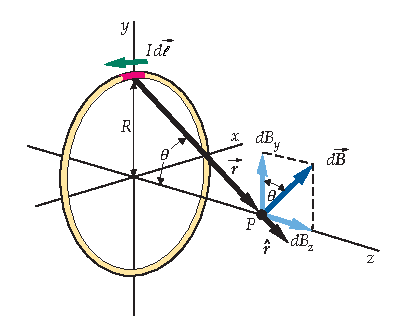
\includegraphics[width=0.55\textwidth]{./images/tip}
\caption{Geometry for calculating the magnetic field at a point on the \textit{z} axis}
\label{F:magneticField}
\end{center}
\end{figure}

	\section{Magnetic Induction}
In the early 1930s Michael Faraday and Joseph Henry independently discovered that in a changing magnetic field a changing magnetic flux through a surface bounded by a closed stationary loop of wire induces a current in the wire \ref{sec:timeline}. This current is also found in a static magnetic field when a changing magnetic flux is created by a moving loop of wire through the surface bounded by the wire itself. 

		\subsection{Magnetic Flux}
The magnetic flux through a surface is the surface integral of the normal component of the magnetic field $\vec{B}$ passing through that surface. In our case these surfaces are defined as the transmitter and receiver coils. As $\vec{B}$ is proportional to the number of field lines per unit area, the magnetic flux is proportional to the number of field lines through an element area \cite{tipler}. Since the coil surface is flat and has a constant area $A$ and several turns $N$, if we assume $\vec{B}$ is uniform in magnitude and direction everywhere on the surface, the magnetic flux through the coil surface is:

  \begin{equation} \label{flux}
    {\phi_m} = \vec{B}\cdot\hat{n}A = NBA\:cos{\theta} 			% Spaces in maths: \,  \:  \;  \!  \(space) \qquad
  \end{equation}

 Where $\theta$ is the angle between the direction of $\vec{B}$ and the direction of the unit vector normal to the coil surface $\hat{n}$.

\begin{figure}[htb]
\begin{center}
	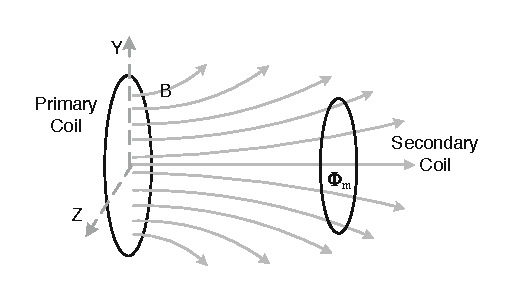
\includegraphics[width=0.7\textwidth]{./images/magneticFlux}
\caption{Magnetic field lines from transmitter to receiver coil}
\label{F:magneticFlux}
\end{center}
\end{figure}

		\subsection{Induced EMF and Faraday's Law}
Equation \ref{flux} shows that flux can be changed by increasing or decreasing $B$, by increasing or decreasing $A$, or by changing the angle ${\theta}$. The idea of changing $A$ or ${\theta}$ is really difficult to achieve and implement compared to changing $B$. Given the magnetic field created by the coil is due to a current in the transmission circuit, the magnitude of the magnetic field can be increased or decreased by increasing or decreasing the current. This change of current will be obtained by using alternating current (AC). The result of this variation of magnetic flux is an emf ${\epsilon}$ induced along the path that is equal in magnitude to the rate of change of the magnetic flux through the surface. This is known as Faraday's law:
  \begin{equation} 
    {\epsilon} = -\frac{d{\theta_m}}{dt}
  \end{equation}

According to the Faraday's law, the polarity of the induced magnetic field is such that it produces a magnetic field opposes the change which produces it. Because the induced voltage and the current are produced at the secondary side, power is successfully transferred from the primary to the secondary side. This is the basic working principles of the inductive coupling.

% begin LLUIS
		\subsection{Inductance}
The simplest way to define what the inductance means is that it is like a resistance but in AC current. It is an opposition to the rate of change of the current. The unit of inductance is the henry (H). As it is shown at follows, one henry is the amount of inductance required to generate one volt when the current is changing at the rate of one ampere per second.
\begin{equation}
{V_L} = L\frac{dI}{dt}
\end{equation}

So it is correct to say that the inductance behaves like a resistance (in AC) because the larger inductance the bigger induced voltage keeping the rate of change of current constant.

In this project are used two types of inductances: the first one, to generate the magnetic flux in one coil, called self-inductance; and the second one, to relate the amount of magnetic flux given by one coil to another coil when they are close enough.

			\subsubsection{Self Inductance}
In this section, the definition of the self-inductance is related to the magnetic field. The reason is because if it is considered a current $I$ going through a coil, this coil generates a magnetic field $B$ that is proportional to $I$\cite{tipler}. The magnetic flux generated by $B$ is also proportional to $I$, as it has expressed in equation \ref{eq:magneticFlux}:
\begin{equation}
\phi_m = L\cdot I
\label{eq:magneticFlux}
\end{equation}

As shown in the previous equation, the inductance $L$ is the proportionality constant and it is called self-inductance. The SI unit of the self-inductance is the henry, as it has said above, and one henry corresponds to one tesla times square meter per ampere.
\begin{equation*}
1\:\textnormal{H} = 1\:\textnormal{T}\cdot\:\textnormal{m}^2/\textnormal{A} = 1\:\textnormal{Wb/A}
\end{equation*}

One possible way to compute the self-inductance of a coil is by calculating, due a knowing current, the magnetic field at every point on the surface bounded by the coil, computing the generated magnetic flux and isolate the self-inductance from the equation \ref{eq:magneticFlux}\cite{tipler}. But the computing of the magnetic field at every point is not a trivial task. Thus, there exist many formulas to easily compute the self-inductance of many types of coils depending on its structure or its geometrical shape, like long solenoids, ferrite-core, air-core and toroid-core inductor, etc. For example, the self-inductance of a long, tightly wound solenoid can be determined by substituting the magnetic flux by the formulas obtained in the electromagnetism theory:
\begin{equation}
\phi_m = NBA = \frac{\mu_0\:N^2\:I\:A}{h}
\end{equation}

where $N$ is the number of turns, and $A$ and $h$ are the coil area and height respectively. If the current flowing through a coil divides the magnetic flux, there is obtained the self-inductance of a long solenoid.
\begin{equation}
L = \frac{\phi_m}{I} = \frac{\mu_0\:N^2\:A}{h}
\end{equation}

These formulas have the characteristic that the value of the coil only depends on the geometrical shape of the coil.
Note that these formulas only depend on the geometrical shape of the coil.

			\subsubsection{Mutual inductance}
Imagine that two or more circuits are close to each other. The amount of magnetic flux through one circuit to the other ones is proportional to the current generated in the first circuit, like the magnetic flux generated by one coil, as we can see in equation \ref{eq:magneticFlux}. The difference is that the proportionality constant is not the self inductance but also is the mutual inductance.

To obtain an expression of the mutual inductance, it is  necessary to know the expression of the magnetic field at a distance $z$. In section \ref{sec:magneticField} it has been determined the equation of computing the magnetic field due to a current loop. This expression can be used for a coil when it is multiplied by $N$ turns. 

Once we have determined the expression of the magnetic field, and considering that two coils are close to each other at a distance $z$, we can obtain an expression of the magnetic flux through the primary coil to the secondary one (equation \ref{flux12}). We will use a similar equation (\ref{flux}) to determine this flux. To simplify the calculations, we are considering that the magnetic flux goes through the perpendicular direction to the area of the primary coil, thus, the value of $cos\:\theta$ becomes one. 

\begin{equation}
\phi_{m12}=M\:I_1\:=\:N_2\:B_1\:A_2
\label{flux12}
\end{equation}

Note that the mutual inductance $M$ is the proportionality constant of the magnetic flux, as it has said above. The equation \ref{eq:magneticField} must be substituted to the equation \ref{flux12} and isolate the mutual inductance.
\begin{equation*}
M=\frac{\mu_0}{2}\:\frac{R_{1}^2\:N_1\:I_1}{(z^2+R_{1}^2)^{3/2}}\:\frac{N_2\:A_2}{I_1}
\end{equation*} \\
\begin{equation}
M=\frac{\mu_0}{2}\:\frac{N_1\:N_2\:R_{1}^2\:R_{2}^2\:\pi}{(z^2+R_{1}^2)^{3/2}}
\end{equation}

As it shows the previous equation, at great distances from the coil, $|z|$ is much greater than $R_1$ and the mutual inductance varies inversely proportional to the distance cubed. This is important to be taken into account because the magnetic flux given by a primary coil to a secondary coil is proportional to the mutual inductance and it will drop rapidly if the distance increases. The conclusion of this is that the closer link distance, the more energy transferred to a secondary coil and a better coupling will be.

	\section{Resonance}\label{sec:resonance}
The resonant circuit, also called LC circuit, can store electrical energy whether it oscillates at its natural frequency (\ref{Eq:naturalFrequency}). The circuit is composed by a coil inductance and a capacitor. The capacitor stores energy in the electric field $E$ between its plates, depending on the voltage across it, and an inductor stores energy in its magnetic field $B$, depending on the current through it. 

		\subsection{Energy Pendulum}
Capacitors and inductors are flip-sides of the same reactive coin, storing and releasing energy in complementary modes. If either the capacitor or inductor starts out in a charged state, by connecting momentarily a battery or by approaching a magnet, the two components will begin to exchange energy between them, back and forth, creating their own AC voltage. 

Frequently, resonance effect is explained using the pendulum analogy comparing the change in kinetic and potential energy to the variation of voltage and current inside the circuit. The pendulum swings at a certain frequency depending on the length of the string holding the mass and not on the mass suspended. In physics, this kind of sine-wave oscillation for a mechanical system is called \textit{Simple Harmonic Motion (SHM)}. The same occurs in the LC circuit where the oscillation and so the frequency are strictly dependent on the sizes of the capacitor and inductor.

\begin{equation}
	\omega_{0} = \sqrt\frac{g}{L}
	\qquad
	\omega_{0} = \frac{1}{\sqrt{LC}}
\label{Eq:naturalFrequency}
\end{equation}

If the power supply frequency for a circuit exactly matches the natural frequency of the circuit's LC combination (Equation \ref{Eq:naturalFrequency}), the circuit is said to be in a state of resonance.

\begin{figure}[ht]
\begin{center}
	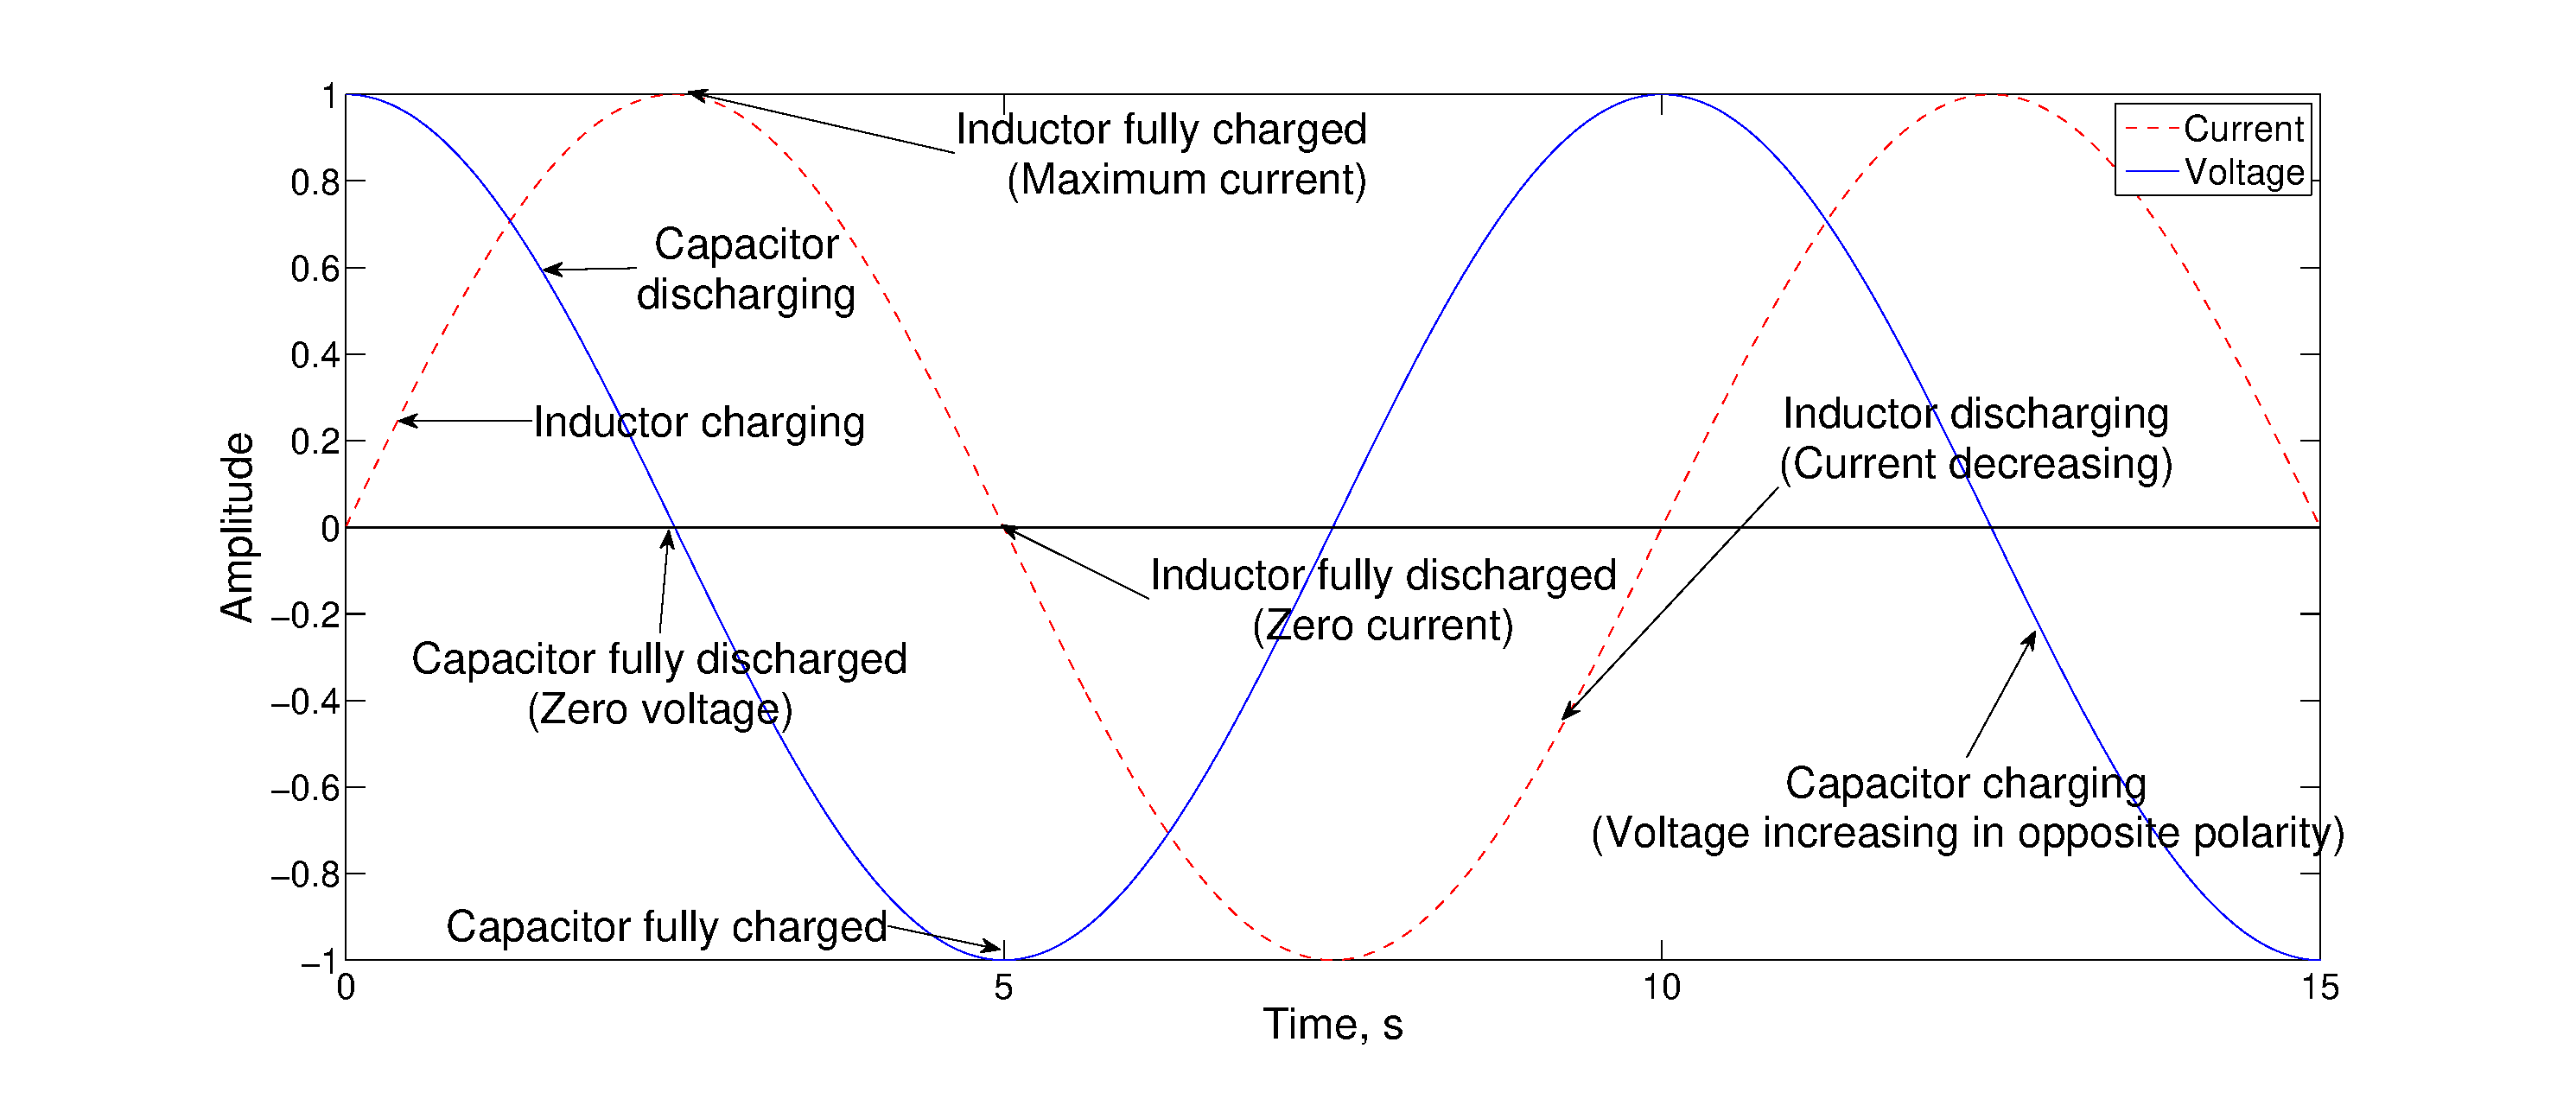
\includegraphics[width=1\textwidth]{./images/VoltageCurrent}
\caption{Voltage and current behaviour inside a LC circuit}
\label{F:VoltageCurrent}
\end{center}
\end{figure}

It can be noticed that there is a phase shift of $90^\circ$ over time between voltage and current measurement in the LC circuit of Figure \ref{F:VoltageCurrent}. This fact will be discussed later. In the same way, whether position and velocity traces of the pendulum were drawn, the same phase shift will be observed.

Both the mechanical and electrical circuits once they have began to oscillate do not last forever. Either resistive or friction losses are the responsible of a finite lifetime.

The pendulum analogy is totally valid for explaining all kind of resonances (e.g., acoustic, mechanical, electromagnetic, etc.) but not enough clear for understanding the resonance between two magnetically coupled resonators. For the purpose of understanding better the behaviour of a coupled system, we think it would be useful to quote the following analogy from F. Hadley\footnote{Franklin Hadley is a Professor with Tenure in the Department of Mechanical Engineering and Materials Science in Duke University.}:

\textit{``Imagine a room with 100 identical wine glasses, each filled with wine up to a different level, so they all have different resonant frequencies. If an opera singer sings a sufficiently loud single note inside the room, a glass of the corresponding frequency might accumulate sufficient energy to even explode, while not influencing the other glasses. In any system of coupled resonators there often exists a so-called `'strongly coupled'` regime of operation. If one ensures to operate in that regime in a given system, the energy transfer can be very efficient.''} 

In our case, the transmitter coil instead of irradiating the environment with electromagnetic waves, it fills the space around it with a non-radiative magnetic field oscillating at a fixed frequency. The non-radiative field mediates the power exchange with the receiver coil, which is specially designed to resonate with the field. The nature of the process ensures a strong interaction between the coils, while minimizing the interaction with the rest of objects \cite{TechTalk}.

The use of resonance results in a much higher efficiency compared to non-resonant inductors, such as typical transformers which require very short range. In addition, by working at the resonant frequency the circuit can achieve its maximum amplitude.

		\subsection{Series Resonance}\label{subsec:seriesResonance}
In order to analyse both series and parallel resonance, a resistance has been added to avoid infinity currents and zero voltage values. These RLC circuits will provide a first approach for understanding the differences when designing the resonant circuit. 

As it is said before, resonance occurs when a series resonant circuit is driven from an external source at a frequency $\omega_0$ at which the inductive and capacitive reactances are equal in magnitude. 

\begin{equation*}
	X_L = X_C
\end{equation*}

This cancellation leaves only the resistance\footnote{An LC circuit is an idealized model since it assumes there is no dissipation of energy due to resistance.} to contribute to the impedance,

\begin{equation*}
	Z_{min} = \sqrt{R^2+(X_L-X_C)^2} = R
\end{equation*}

The impedance is also at a minimum at resonance (see Figure \ref{F:series1}). Below that natural frequency, called resonant frequency $\omega_{res}$, the series resonant circuit looks capacitive since the impedance of the capacitor increases while inductive reactance is decreasing. Above resonance the circuit behaves oppositely.

\begin{figure}[h!]
  \begin{center}
    \begin{circuitikz}
    \ctikzset{v/.append style={/tikz/american voltages}}
    \ctikzset{bipoles/resistor/height=0.25}
    \ctikzset{bipoles/resistor/width=0.7}
      \draw (0,0)
      to[sinusoidal voltage source,v=$V_{S}$] (0,3)
      to[short] (1,3)
      to[C=$C$] (2,3)
      to[short] (3,3)
      to[L=$L$] (4,3)
      to[short] (5,3)
      to[R=$R$,v_=$V_R$,-] (5,0)
      to[short] (0,0);

    \end{circuitikz}
    \caption{Series resonance}
  \end{center}
\end{figure}

At resonance frequency, due to the smallest circuit impedance, the current is greatest, 

\begin{equation}
	I_{max} = \frac{V}{Z_{min}}
\end{equation}

Thus, resonant current peak is set by the resistor value.

\begin{figure}[htb]
\begin{center}
\begin{subfigmatrix}{2} 
\subfigure[Impedance and reactance w.r.t. frequency] % With Respect To
	{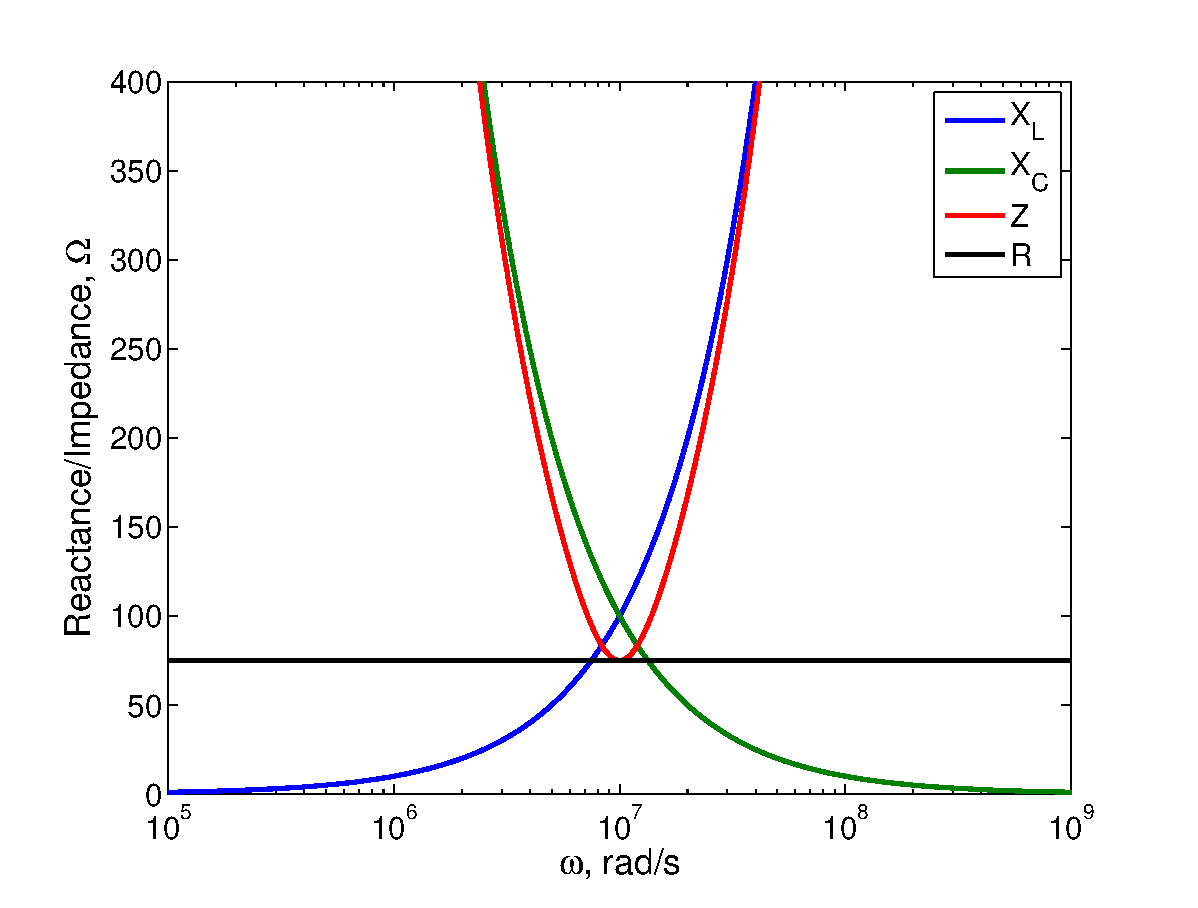
\includegraphics{./images/series1}\label{F:series1}} 
\subfigure[Voltage gain in the resistor]
	{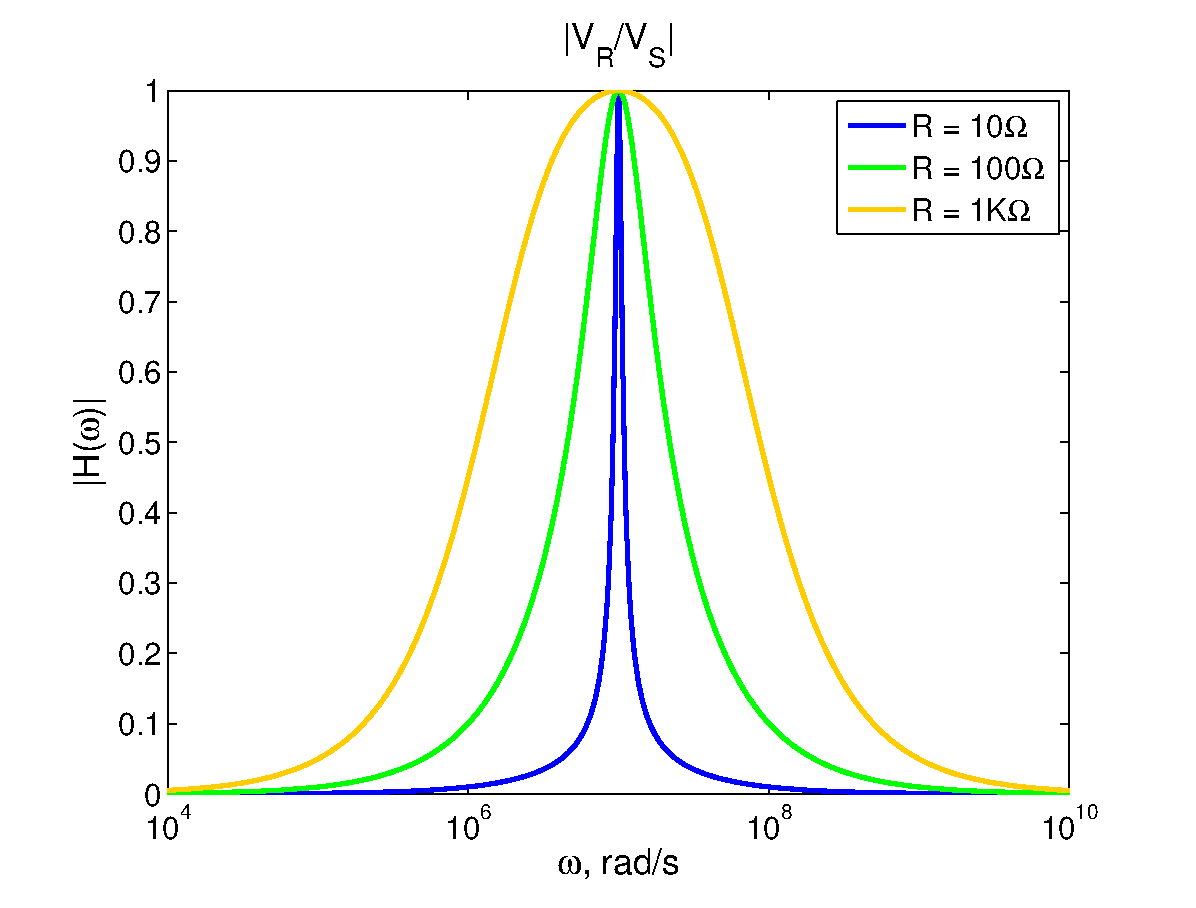
\includegraphics{./images/series2}\label{F:series2}}
\end{subfigmatrix}
\caption{Series RLC circuit}
\label{F:seriesRLC}
\end{center}
\end{figure}

		\subsection{Parallel Resonance}
In the same way as series resonance, the parallel resonant circuit is purely resistive at $\omega_{res}$, where $X_L = X_C$. 


\begin{figure}[hbt]
  \begin{center}
    \begin{circuitikz}
    \ctikzset{v/.append style={/tikz/american voltages}}
    \ctikzset{bipoles/resistor/height=0.25}
    \ctikzset{bipoles/resistor/width=0.7}
      \draw (0,0)
      to[sinusoidal voltage source,v=$V_{S}$,i^=$i_S$] (0,3)      
      to[short] (3,3)
      to[C=$C$] (3,0)
      to[short] (0,0);
      \draw (3,3)
      to[short] (5,3)
      to[L=$L$] (5,0)
      to[short] (3,0);
      \draw (5,3)
      to[short,i=$i_R$] (7,3)
      % to[short,i=$i_R$] (7,2)
      to[R=$R$] (7,0)
      to[short] (5,0);
    \end{circuitikz}
    \caption{Parallel resonance}
  \end{center}
\end{figure}

This time the parallel RLC circuit has a current gain rather than a voltage gain. Its impedance is maximized at the resonant frequency rather than minimized.

Below this frequency, the resonant circuit looks inductive since the impedance of the inductor is lower. Above resonance, the capacitive reactance decreases. In both cases the current drawn is larger than the current at resonance case \cite{aacResonance}. In both parallel and series circuits, the resonant frequency remains the same.

\begin{figure}[htb]
\begin{center}
\begin{subfigmatrix}{2} 
\subfigure[Impedance and reactance w.r.t. frequency] % With Respect To
	{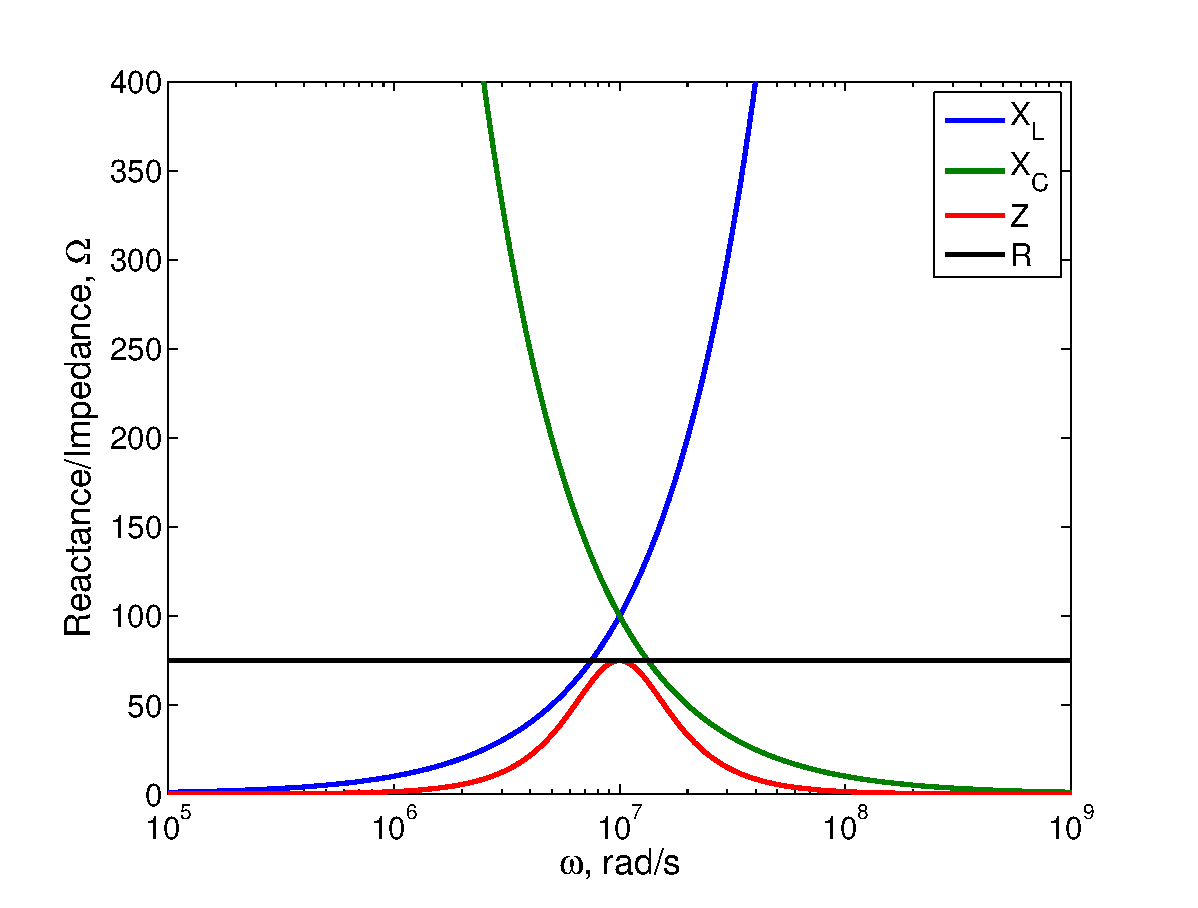
\includegraphics{./images/parallel1}\label{F:parallel1}} 
\subfigure[Current gain in the resistor]
	{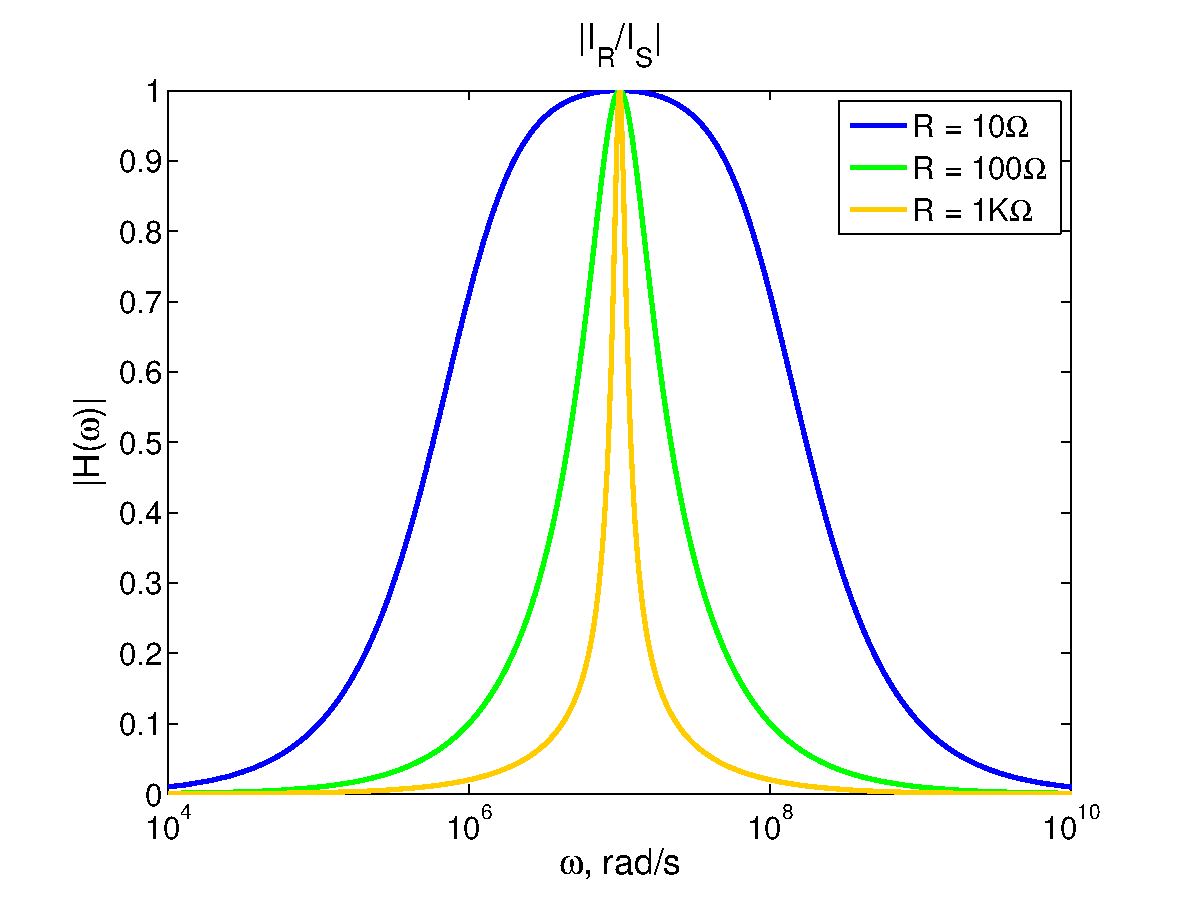
\includegraphics{./images/parallel2}\label{F:parallel2}}
\end{subfigmatrix}
\caption{Parallel RLC circuit}
\label{F:parallelRLC}
\end{center}
\end{figure}

Figure \ref{F:parallel1} shows how impedance is at a peak at resonant frequency and therefore voltage is maximum. The reason for this is that voltage is proportional to impedance. 

\begin{equation}
	V = I\cdot{Z}
\end{equation}

 % This is satisfactory if the resistances are small (http://hyperphysics.phy-astr.gsu.edu/hbase/electric/parres.html)

	\section{Characterizing the Inductor} %Coil Modeling
In order to transfer power wirelessly, the LC-pair is adopted because it is the oldest and most frequently used technique. It is rapidly assembled by winding a \textit{piece} of wire and placing a capacitor either in series or parallel, depending on the desire effect. The capacitor is adopted at both side to keep the coils resonate at the designed frequency.

There are many ways to model a coil. Figure \ref{F:modelingCoil} shows one of them, composed by the coil inductance $L$ itself and a coil conductor resistor $R$. This resistance is placed to quantify \textit{Copper loss} or winding loss which is the term used to describe the energy dissipated by resistance in the wire used to wind the coil \cite{CopperLoss}. There is also an equivalent parasitic capacitor $C_{p}$ connected to the inductor and resistor. This parasitic capacitance is due to the fact that the inductor is made out of a coil of insulated wire. Therefore, tiny capacitors are created between the windings since there are two sections of wire separated by an insulator. 

Another simplified equivalent circuit is shown on the right in Figure \ref{F:modelingCoil}. The impedance of the coil is represented by a real impedance component $Re$ and an imaginary impedance component $Im$ (impedance equations are presented in Appendix \ref{AppendixSection: impedance}). This modeling approach has been verified, especially in the low frequency range\cite{medical}. For high-accuracy applications, like PCB spiral coils, complex models \cite{Eddy} can be used. 

\begin{figure}[h]
\begin{center}
	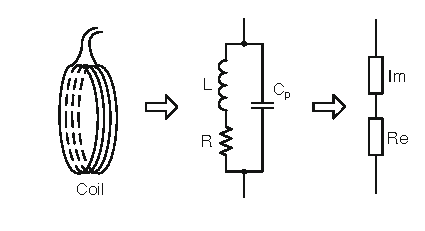
\includegraphics[width=0.7\textwidth]{./images/med}
\caption{Modeling of a single magnetic coil}
\label{F:modelingCoil}
\end{center}
\end{figure}

		\subsection{Coil Resistance}\label{subsec:coilResistance}
The calculation of the resistance of a coil is important because it limits the power transferred in a WPT system. If the resistances of a coil were zero, the power transfer efficiency would be 100$\%$, and there would not exist any limitation to transfer energy at a given distance. However, the ideal world does not exist and appear resistances that generate heat due to Joule effect: power losses. The goal of a WPT system is to minimize this power losses to ensure the maximum transferred power and efficiency.

\subsubsection{DC Resistance}
At low frequencies ($f<$ 200 kHz) \cite{meyer} the resistance experiments a DC behavior. The value of this resistance does only depend on the wire geometry and material. The DC resistance of a metal conductor is given by \cite{medical}

\begin{equation}
R_{DC}=\rho\:\frac{l}{S}
\label{DCres}
\end{equation}

where $l$ is the wire length in meters, $S$ is the wire section in square meters and $\rho$ is the electrical resistivity of the metal material, measured in $\Omega\cdot$m. In table \ref{T:electricalResistivity} are exposed different electrical resistivities for some metal conductors.

\subsubsection{AC Resistance}
When the frequency increases up to 200 kHz we can not talk anymore about DC resistance, the reason is the appearance of some effects that increase the wire resistance with the frequency. From now on, the resistance will behave as an AC resistance due to the \textit{skin-effect} and \textit{proximity-effect}. 

\textit{Skin-effect} happens in all wire and cable. When the signal is DC, it uses the entire conductor, with the same amount of current flowing in the center of the wire as on the outside. As the frequency is increased, the current density begins to move further away from the conductor that inside it. Consequently, the equivalent cross section of the conductor decreases and as Figure \ref{F:skinDepth} shows, the wire resistance is increased with frequency. To quantify the \textit{skin-effect} it is introduced the skin depth $\delta$. Skin depth is a measure of how far electrical conduction takes place in a conductor, and is a function of frequency, no matter how thick the wire is. It is calculated as described below \cite{mit2},


\begin{equation}
% \delta=\sqrt{\frac{2\:\rho}{\omega\:\mu}}
\delta = \frac{1}{\sqrt{\pi{f}\mu\:\sigma}}
\end{equation}

where $\sigma$ is the electrical conductivity of the wire material ($\sigma_{copper}=5.8 \text{ x } 10^7$ S/m), $f$ is frequency in Hz and $\mu$ is the total permeability defined as the permeability in free space times the material permeability ($\mu=\mu_0\cdot{\mu_m}$). 

Owing to skin depth decreases with respect to the frequency as a negative exponential, conductors can become thinner at higher frequencies with little impact on circuit loss, because skin depth shrinks with frequency. A rule of thumb is always plan on providing at least five skin depths of low-loss conductor in order to provide good performance without the need of invest better conductors \cite{skinDepth}. This effect can be reduced by using \textit{Litz wire} \cite{ACres}.

The resistance corresponding to  \textit{skin-effect} can be determined in the following way:

\begin{equation}
R_{skin}=R_{DC}\:\frac{4\:d}{\delta}
\end{equation}

The $R_{skin}$ is the result of multiplying the $R_{DC}$ by the coefficient $4d/\delta$, which is proportional to the square root of the frequency.

\begin{figure}[htb]
\begin{center}
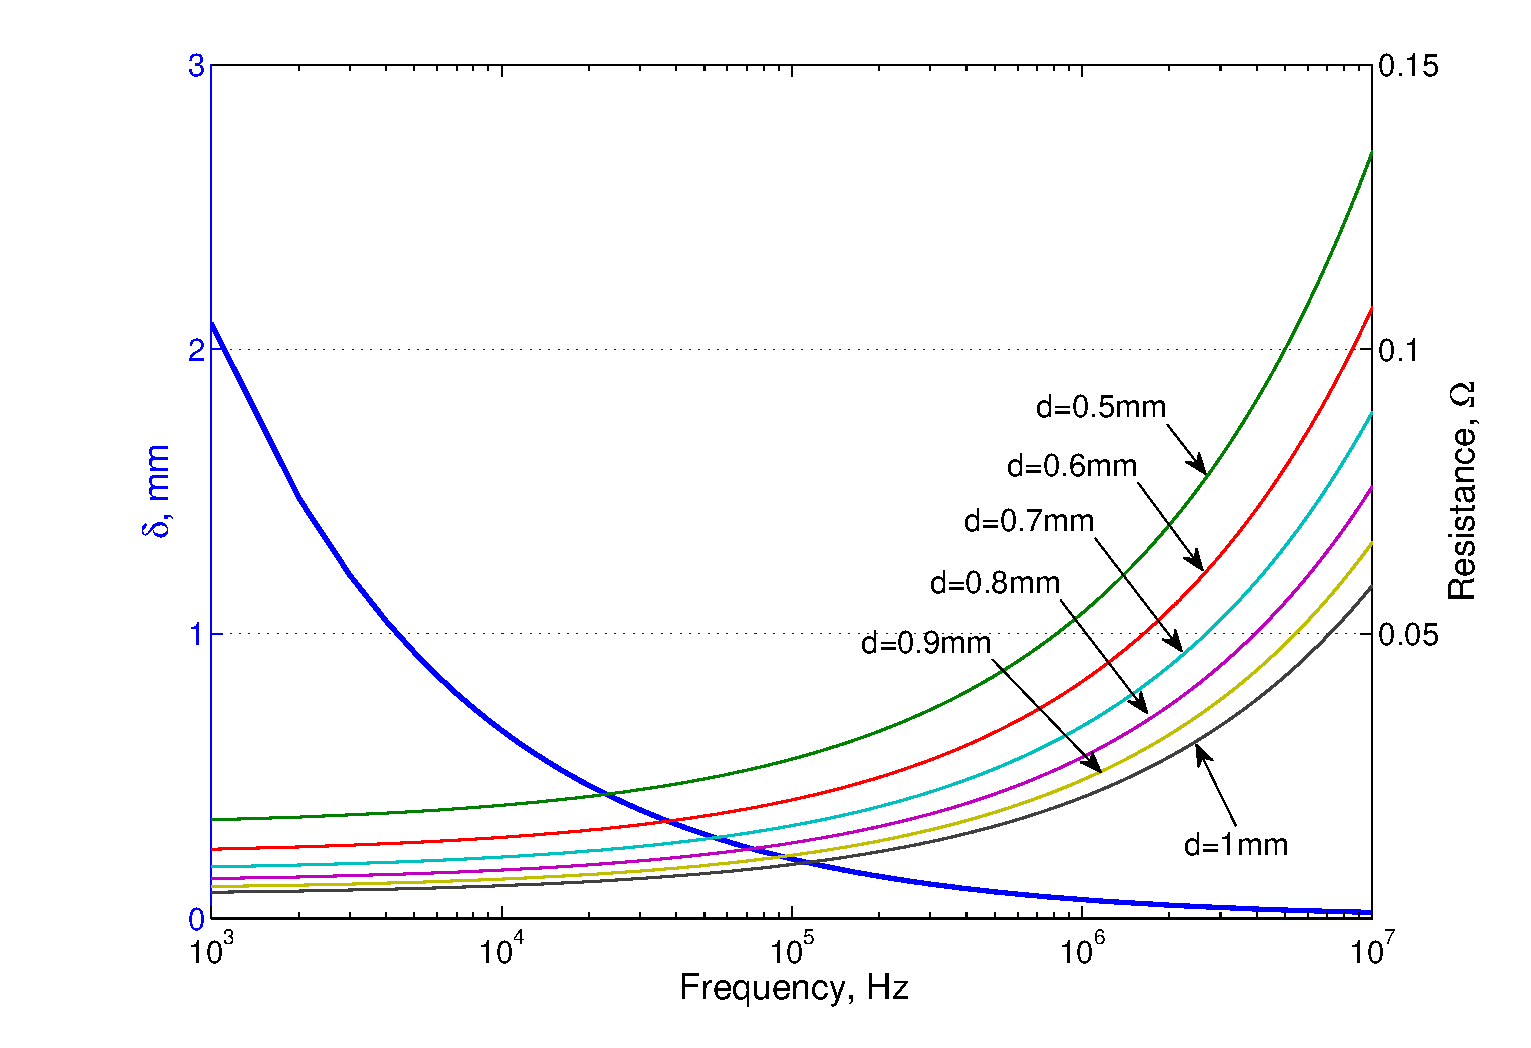
\includegraphics[width=0.7\textwidth]{./images/skinDepth}
\caption{Skin depth and resistance varying frequency for a fixed coil}
\label{F:skinDepth}
\end{center}
\end{figure}

Besides the \textit{skin-effect} there is another phenomena that increase the resistance value of a conductor when is applied an alternating current, called \textit{proximity-effect}. This effect is the apparent increase in the resistance of the wire due to the circulating current in the conductor caused by the alternating flux of the other nearby conductors. As a result, more power losses in the windings appear. To quantify the \textit{proximity-effect}, there is used the Dowell's assumption \cite{ACres}:
\begin{equation}
R_{proximity} = R_{DC}\:\psi\:\left [ \frac{sinh(2\:\psi)+sin(2\:\psi)}{cosh(2\:\psi)-cos(2\:\psi)}+\frac{2}{3}(m^2-1)\frac{sinh(2\:\psi)-sin(2\:\psi)}{cosh(2\:\psi)+cos(2\:\psi)} \right ]
\end{equation} 

In the above equation, the parameter $\psi$ can be determined in the following form:
\begin{equation*}
\psi = \left ( \frac{100\:d}{2\:\delta} \right )\:\sqrt{\pi}
\end{equation*}

Here, $m$ indicates the number of layers, and $\delta$ is the skin depth previously mentioned.

To conclude this section, the total equivalent series resistance $R_{ES}$ that appears when an alternating current flows through a wire is the sum of all these effects in addition to the ``parasitic'' resistance of the wire, called DC resistance. 

\begin{equation}\label{eq:Resistance}
R_{ES} = R_{DC}+R_{skin}+R_{proximity}
\end{equation} 
%%%%%%%%%%%%%%%%%%%%%%%%%
% Resistencia radiación %
%%%%%%%%%%%%%%%%%%%%%%%%%

		\subsection{Coil Inductance}\label{subsec:coilInductance}
In this project air-core inductors are required due their low weight compared to solid-core, despite the last provide better coupling. The reason of avoiding better \textit{transformers}, as it said in previous sections, is that the primary coil is wanted to go on a nano-quadcopter. Thus, the most typical formulas to compute the self-inductance of an air-core inductor are exposed below.

The most typical formula that is used in many projects or studies is the equation of a circular loop coil \cite{TypicalL},\cite{UAV},\cite{Melliptical}:

\begin{equation}\label{Eq:typical}
L=\mu_0\:R\:N^2\:(ln\frac{8R}{d/2}-1.75)\qquad [\textnormal{H}]
\end{equation}

where $d$ is the wire diameter.

Another equation is the Harold A. Wheeler’s formula to compute the inductance for a finite-length solenoid:
\begin{equation}\label{Eq:Harold}
L=\frac{N^2\:R^2}{9R+10h}\qquad [\mu \textnormal{H}]
\end{equation}

The units of length are expressed in inches. This formula is correct to within 1 per cent for coils with $h>0.8R$ \cite{wheeler}.

Similar to the Harold A. Wheeler’s formula, an equation for air-cored inductor is exposed below \cite{WaiKaiChen}:
\begin{equation}\label{Eq:Wai}
L=2\:K\:R\:N^2\qquad [\mu \textnormal{H}]
\end{equation}

where $K$ is a parameter that depends on the dimension ratio ($D/h$) of the coil, whose values are listed in Appendix \ref{Appendix: AA} and the units of length in this equation are expressed in centimeters.












		\subsection{Coil Parasitic Capacitor}
Every coil has a parasitic capacitor. Since the inductor is made out of a coil of insulated wire, tiny capacitors between the windings are created. This is due each section of windings is at a slightly different potential because of wire inductance and resistance. When the current frequency is high enough, most current in the coil would be bypassed via the parasitic capacitor \cite{medical}. As a result, the coil can not be viewed as a lumped inductor anymore. The coil's inductance would resonate with the parasitic capacitor at a frequency. This frequency is called the self-resonant frequency ($f_s$).

\begin{equation}
	f_{s} = \frac{1}{2\pi\sqrt{LC_{par}}}
\end{equation}

The parasitic capacitance is connected in parallel to the inductor and the resistor. Its value is relatively small, of the order of 1 pF, which is insignificant at low frequencies but not at very high frequencies ($>$ 5 MHz) \cite{tesis}. Because of this capacitance, the coil has a self-resonance frequency between 10 MHz and 25 MHz.

The parasitic capacitance effect can be alleviated by keeping inductor windings far apart, and so reducing the capacitance by using helical coils. The second option to reduce parasitic capacitors is to work at a frequency low enough. This frequency will be discussed in Section \ref{subsec:operatingFreq}. For the following theorical model parasitic capacitors will be disregarded.

	\section{Coreless Transformer Modeling}
In this section the electrical model of the resonant magnetic induction system will be determined by using the air coreless transformers theory, in which WPT systems are based on. It is called transformer because it transforms electrical energy into magnetic energy, then back into electrical energy again. Because its operation depends on electromagnetic induction between two stationary coils and a magnetic flux and polarity, transformers are necessarily AC devices. 














\begin{table}[h]
\begin{center}
\begin{tabular}{|c|c|}

\noalign{\global\arrayrulewidth1pt}
\hline
\textbf{Parameter} 	& 	\textbf{Definition}\\
\hline
\hline
$V_S$ 		& Source voltage		\\ \hline 
$I_1$  		& Primary current		\\ \hline 
$I_2$  		& Secondary current		\\ \hline 
$R_1$  		& Primary resistance	\\ \hline 
$R_2$ 		& Secondary resistance	\\ \hline 
$R_L$		& Load resistance		\\ \hline
$L_1$		& Primary inductance 	\\ \hline
$L_2$		& Secondary inductance 	\\ \hline
$C_1$		& Primary capacitor 	\\ \hline
$C_2$		& Secondary capacitor 	\\ \hline
$M$			& Mutual inductance 	\\ \hline
$\omega$	& Angular frequency 	\\ \hline     
\end{tabular}
\caption{Electric parameters}
\label{T:Electric parameters}
\end{center}
\end{table}

% Its working principle consists in appliying a high frequency current in the transmitter coil. Hence, only a percentage of the alternating magnetic flux created will penetrate the receiver coil. Thus, a voltage is induced in the receiver side due to magnetic induction.      

		\subsection{Electrical Circuit} \label{subsec:Model}
In the first analysis, the  electric system of non-resonant induction is discussed in a generic way. A typical inductive system consists of a primary transmitter coil (\textit{Tx}) and a secondary receiver coil (\textit{Rx}), but there can be added more coils to the system.

The \textit{Tx} coil is characterized by a winding that has a resistance $R_1$ and an inductance $L_1$. Similarly, the secondary coil \textit{Rx} is characterized by a winding resistance, $R_2$ and an inductance, $L_2$.

\begin{figure}[ht!]
  \begin{center}
    \begin{circuitikz}
    \ctikzset{bipoles/resistor/height=0.25}
    \ctikzset{bipoles/resistor/width=0.7}
     \draw (0,0)
     to[sinusoidal voltage source,v=$V_S$] (0,4) 
	 to[short] (1,4) 
	 to[R=$R_1$] (2,4) 
	 to[short] (3,4)
     to[L=$L_1$] (4,4)
     to[short] (5,4);
     \draw (0,0) 
     to[short] (5,0)
     to[sinusoidal voltage source,v=$jwMI_2$] (5,4);
     \draw (6,0) 
     to[sinusoidal voltage source,v_=$jwMI_1$] (6,4)
     to[short] (7,4)
     to[L=$L_2$] (8,4)
     to[short] (9,4)
     to[R=$R_2$] (10,4)
     to[short] (11,4)
     to[generic=$R_L$] (11,0)
     to[short] (6,0);
      \draw[thin, <-, >=triangle 45] (2,2)node{$i_1$}  ++(-60:0.8) arc (-60:170:0.8);
      \draw[thin, <-, >=triangle 45] (9,2)node{$i_2$}  ++(-60:0.8) arc (-60:170:0.8);
    \end{circuitikz}
   \caption{General electric circuit}
\label{F:Electric}
  \end{center}
\end{figure}
As it can be seen in Figure \ref{F:Electric}, the system does not include compensation capacitors neither in the transmission side nor the reception. Thus, a non-resonant\footnote{Note this is stated for ideal coils which need of a compensation to become resonant.} is studied on a first approach. The system is excited by a perfect sine wave in steady state condition. For simplicity, the lumped element model is assumed regarding that $\lambda$ is much bigger than the characteristic length of the circuit. This assumption declares that all circuit elements, such as resistors, inductors and capacitors, are concentrated into idealized electrical components.

The circuit model offers a convenient way to systematically analyze the characteristic of the system \cite{matrix}. By applying circuit theory Kirchhoff's Voltage Law (KVL) to this system a relationship between currents through each coil and the voltage applied to the transmitter coil can be described as the following equation system:

\begin{numcases}{}
	V_S=R_1\cdot{I_1}+j\omega{L_1}\cdot{I_1}-j\omega{M}\cdot{I_2} \label{eq1}
\\
	0 = R_2\cdot{I_2}+R_L\cdot{I_2}+j\omega{L_2}\cdot{I_2}-j\omega{M}\cdot{I_1} \label{eq2}
\end{numcases}

These equations show how the primary side induces voltage into the secondary side which depends on the frequency, mutual inductance and the primary coil's current, which is also called magnetizing current since it is the responsible of generating the magnetic field and so the magnetic flux.

The system of linear equations can be arranged as the following symmetric matrix \ref{M:kvl}.  

\begin{equation}
\begin{bmatrix}
    V_{S} 	\\
    0 		\\
\end{bmatrix}
=
\begin{bmatrix}
    Z_{1} 			& -j{\omega}M  	\\
    -j{\omega}M 	& Z_{2}  		\\
\end{bmatrix}
\begin{bmatrix}
    I_{1}	\\
    I_{2}	\\

\end{bmatrix}
\label{M:kvl}
\end{equation}

In order to transfer the maximum power and reduce losses the proposed model is based on \cite{meyer}, which defines an equivalent impedance matching method. The procedure analyses the effect of the complete secondary circuit on the primary side. Thus, the secondary circuit is viewed from the voltage supply as a reflected impedance $Z_R$.

Firstly, the secondary current will be isolated from the Equation \ref{eq2}, becoming:

\begin{equation}
	I_2 = \frac{j\omega{M}}{R_2+R_L+j\omega{L_2}}\cdot{I_1}
\end{equation}

To determine the expression of $Z_R$, all the secondary-side components, including the load resistance $R_L$, can be gathered into a single impedance expresion called secondary impedance $Z_2$:

\begin{equation}
	Z_2 = R_2+R_L+j\omega{L_2}
\end{equation}

In the same way, the primary circuit impedance is defined in the next manner:

\begin{equation}
	Z_1 = R_1+j\omega{L_1}
\end{equation}

Now, the current at secondary circuit can be expressed as:

\begin{equation} \label{eq:I2}
	I_2 = \frac{j\omega{M}}{Z_2}\cdot{I_1}
\end{equation}

Substituting $I_2$ in Equation \ref{eq2}, we are forcing voltage source to ``see'' secondary circuit as a single impedance, $Z_R$.

\begin{equation} \label{Eq:ZR}
	V_S = Z_1\cdot{I_1}+\frac{\omega^2{M^2}}{Z_2}\cdot{I_1} 
\end{equation}

where $Z_R$ is defined as:

\begin{equation}
	Z_R = \frac{\omega^2M^2}{Z_2}
\end{equation}

Thereby, equation \ref{Eq:ZR} is rearranged in the form:

\begin{equation}
	V_S =(Z_1+Z_R)\cdot{I_1}
\end{equation}

To simplify even more the expression, it is possible to define the whole circuit as the following single impedance (see Figure \ref{F:equivalentCircuit}):

\begin{equation}
	V_S = Z_{eq}\cdot{I_1}
\end{equation}


\begin{figure}[ht!]
  \begin{center}
    \begin{circuitikz}
	\ctikzset{v/.append style={/tikz/american voltages}}
    \ctikzset{bipoles/resistor/height=0.25}
    \ctikzset{bipoles/resistor/width=0.5}
     \draw (0,0) 
     to[sV,v=$V_S$] (0,4) 
	 to[short] (1,4) 
	 to[R=$R_1$] (2,4) 
	 to[short] (3,4)
     to[L=$L_1$] (4,4)
     to[short] (5,4);
     \draw (5,0) 
     to[generic=$Z_R$] (5,4);
	\draw(5,0)
	to[short] (0,0);
     % to[short] (0,5);
     \draw(5,3) node[anchor=west] {+};
	 \draw (5,1) node[anchor=west] {-};
	 \node at (5.75,2) {$V_{out}$};
    \end{circuitikz}
   \caption{Reflected impedance circuit schematic}
\label{F:reflectedCircuit}  
\end{center}

\end{figure}

\begin{figure}[ht!]
  \begin{center}
    \begin{circuitikz}
	\ctikzset{v/.append style={/tikz/american voltages}}
    \ctikzset{bipoles/resistor/height=0.25}
    \ctikzset{bipoles/resistor/width=0.5}
	\draw (0,0) 
     to[sinusoidal voltage source,v=$V_S$] (0,4) 
	 to[short] (5,4);
     \draw (0,0)
     to[short] (5,0)
     to[generic=$Z_{eq}$] (5,4);
	\draw(5,3) node[anchor=west] { };
	 \draw (5,1) node[anchor=west] { };
	 \node at (5.75,2) {$\qquad$};
    \end{circuitikz}
   \caption{Equivalent impedance circuit schematic}
\label{F:equivalentCircuit}  
\end{center}

\end{figure}

Once the $Z_R$ is determined, it is possible to calculate the voltage drop across it by using the voltage divider expression:

\begin{equation}
	V_{out} = V_S\cdot\frac{Z_R}{Z_R+Z_1}
	\label{eq:vout}
\end{equation}

Hence, the power transferred to the reflected impedance is given by:

\begin{equation}
	P_{out} = \frac{V_{out}^2}{Z_{R}}
\end{equation}

Replacing $V_{out}$ for the expression \ref{eq:vout}, the power at the reflected impedance only depends on the source voltage (also called $V_{in}$).

\begin{equation}
	P_{out} = V_{in}^2\cdot\frac{Z_R}{(Z_1+Z_R)^2}
\end{equation}

For the fixed value of $Z_1$, it is found the optimal $Z_R$ value computing the partial derivative of $P_{out}$ with respect to $Z_L$.
\begin{equation}
	P_{out_{max}}\Rightarrow\frac{dP_{out}}{dZ_R}=\frac{(Z_1+Z_R)^2-2\cdot{Z_R}\cdot(Z_1+Z_R)}{(Z_1+Z_R)^4}=0
\end{equation}

It is found that the maximum power transfer occurs when $Z_R=Z_1$. This results in a restrictive parameter since $Z_R$ depends on the mutual inductance which in turn depends on the distance between the transmitter and receiver coil. Thus, there is no a unique optimal value of $Z_R$. 

In order to discuss the air-core transformer, the general non-resonant system has been introduced. This system has an important energetic drawback. Secondary coil impedance is used to be high. Hence, it is the responsible for a significant current drop in the load resistance \ref{eq:I2} \cite{meyer}. Whether the power transferred to the load is intended to be increased, at first sight, the input voltage should be also increased owing to $P_{out}$ is proportional to the square of $V_{in}$. But this solution is not optimal at all because it requires higher current amplitudes in the primary coil, and therefore greater Joule losses.

In the following section, resonance capacitors will be added to the primary and secondary circuits. They will cancell (or decrease notably) the large reactance of a coil by working at the resonant frequency. These capacitors allow to reduce the current amplitudes and, as a result, to improve the efficiency of the coreless transformer. 




%%% LLUIS
\subsection{Compensation Topologies}
As it is said in Section \ref{sec:resonance}, the transmitting and receiving coils are designed to operate at the resonant frequency to establish an efficient energy channel for power transfer. This is done by using compensation capacitors. Here, the four typical resonant configurations are discussed, which are labeled as SS, SP, PS and PP. The first S or P indicates series or parallel for the primary capacitors and the second S or P means the same for the secondary capacitor. Depending on the resonant type, if the primary capacitor is in series, the transmitting coil will be driven by an AC voltage source, and, whether it is in parallel, the transmitting coil will be driven by an AC current source \cite{matrizNegativa}.

\begin{figure}[htb]
\begin{center}
\begin{subfigmatrix}{2} 
\subfigure[SS]
{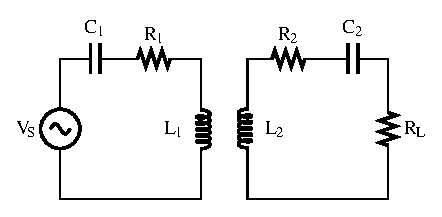
\includegraphics{./images/SS}\label{F:SS}} 
\subfigure[SP]
{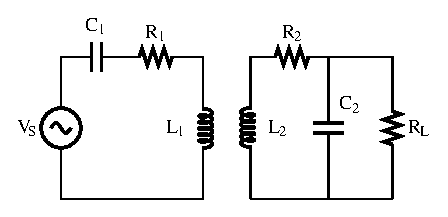
\includegraphics{./images/SP}\label{F:SP}}
\subfigure[PS] 
{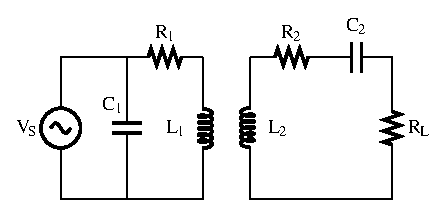
\includegraphics{./images/PS}\label{F:PS}} 
\subfigure[PP]
{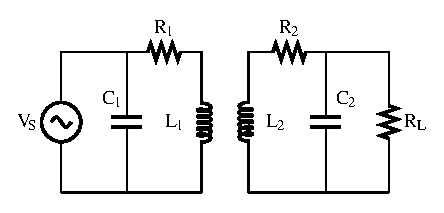
\includegraphics{./images/PP}\label{F:PP}}
\end{subfigmatrix}
\caption{Compensation topologies}
\label{F:topologies}
\end{center}
\end{figure}

In this section each topology is evaluated in a detailed way to determine their advantages and drawbacks, and then, to conclude which is the most suitable topology according to our application. Therefore, the equations determined in Section \ref{subsec:Model} will be changed due to the insertion of the compensation capacitors, depending on the used topology. This new equations are listed in Appendix \ref{Appendix: A}. 

Eventually the best topology in terms of maximum transferred power will be chosen. Arbitrary values are selected from the system parameters represented in Table \ref{T:ArbitraryValues}. 

\begin{table}[h]
\begin{center}
\begin{tabular}{|c|c|}

\noalign{\global\arrayrulewidth1pt}
\hline
\textbf{Parameter} & \textbf{Value}\\
\hline
\hline
$V_S$ 	& 5 V\\ \hline 
$R_S$   & 50 $\Omega$\\ \hline
$R_1$   & 0.5 $\Omega$\\ \hline
$R_2$ 	& 0.5 $\Omega$\\ \hline
$R_L$ 	& 50 $\Omega$\\ \hline
$L_1$ 	& 10 $\mu$H \\ \hline
$L_2$ 	& 10 $\mu$H \\ \hline
$C_1$ 	& 2 nF \\ \hline
$C_2$ 	& 2 nF \\ \hline
$M$ 	& 3 $\mu$H \\ \hline     
\end{tabular}
\caption{Arbitrary values of the electric parameters}
\label{T:ArbitraryValues}
\end{center}
\end{table}


All the calculations for computing the efficiency and the output power (load power) are done using the alternating current basics. Thus, the input power $P_{in}$ and the load power $P_{L}$ are given by,

\begin{equation}
P_{in} = V_{in}\cdot{I_{in}}\cdot{cos(\varphi)}
\end{equation}

\begin{equation}
P_{L} = ( I_{L} ) ^2\cdot{R_L}
\end{equation}

where $\varphi$ is the phase between the input voltage and the primary current. In the previous equations, it is used the root mean square (\textit{RMS}) for $V_{in}$, $I_{in}$ and $I_L$; as a consequence, the power results are expressed in its average value.  Note that $P_{in}$ is multiplied by the power factor $cos(\varphi)$ which corresponds to compute the active power or consumable power.

\subsubsection{SS topology}

The equivalent circuit of the SS topology can be determined by gathering the expression of $Z_R$ with $Z_{eq}$ listed in Appendix \ref{sec:secondaryS} and \ref{sec:primaryS} respectively. By varying the frequency, the efficiency $\eta$ and the output power (load power) will show their maximum at the resonance frequency. 

In Figure \ref{F:effTopologies}, when the frequency grows, the efficiency tends to a constant value that depends on the system parameters. This statement does not mean that is optimal to work at high frequencies because the output power drops sharply when the frequency overtakes the resonance frequency. The explanation is that the input power also falls with the same magnitude as the output power.

Another interesting parameter for studying in each topology is the equivalent impedance of the system. This impedance will help us to determine the optimal compensation for our application because its behavior depends on the operating frequency. Figure \ref{F:SSimpedance} shows that at the resonance frequency, the whole imaginary part of $Z_{eq}$ is canceled and the system impedance is purely resistive. The impedance of this compensation topology behaves as a capacitance since the the frequency increases to the resonance frequency; from this point, it will behave as an inductance.


\begin{figure}[h!]
\begin{center}
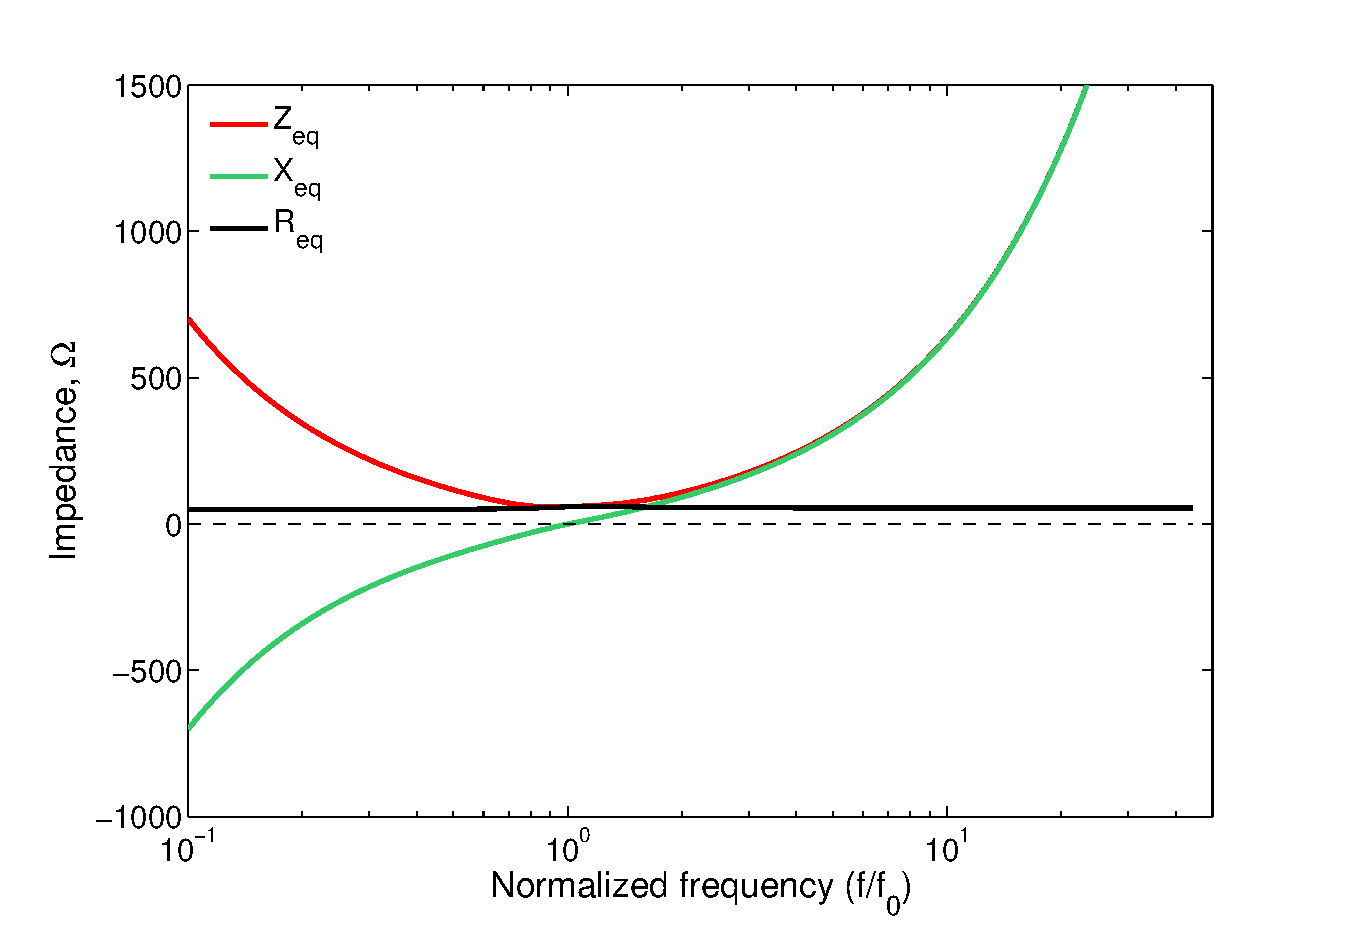
\includegraphics[width=0.7\textwidth]{./images/SS_impedance} 
\caption{Equivalent circuit impedance w.r.t frequency for SS topology}
\label{F:SSimpedance}
\end{center}
\end{figure}

% \\
\subsubsection{SP topology}

It is possible to model the SP topology using the formulas obtained for $Z_R$ and $Z_{eq}$ in Appendix \ref{sec:secondaryP} and \ref{sec:primaryS} respectively. As it is explained in Appendix \ref{sec:secondaryP}, to transfer the maximum power to the system load, is recommended to delete the imaginary part of $Z_R$. This is done by changing the secondary capacitor value to a value that can be computed using the Equation \ref{Eq:differentCapacitor}, allowing to transfer only consumable power to the load. As a consequence, the maximum efficiency and load power will be at a different frequency than the resonance frequency of the whole system\footnote{The system resonance frequency in this case will be a trade-off between the resonance frequency of both primary and secondary circuits due to the different capacitance used.}. The impedance's model has a similar curve as in case of the SS topology impedance as Figure \ref{F:SPimpedance} shows.

\begin{figure}[h!]
\begin{center}
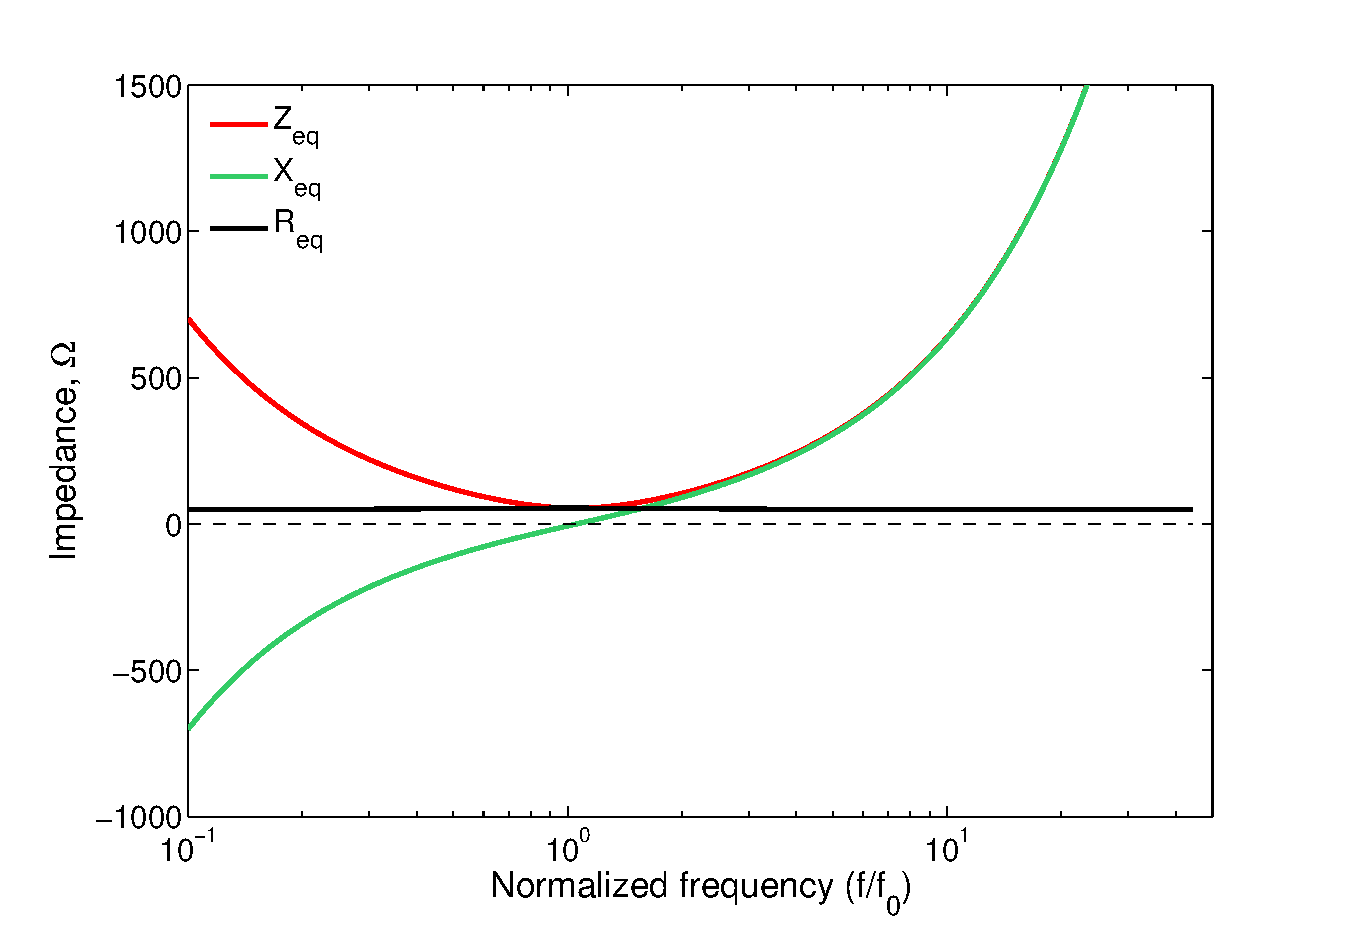
\includegraphics[width=0.7\textwidth]{./images/SP_impedance} 
\caption{Equivalent circuit impedance w.r.t frequency for SP topology}
\label{F:SPimpedance}
\end{center}
\end{figure}

\subsubsection{PS topology}

The SP topology are modeled with the equations for $Z_R$ and $Z_{eq}$ listed in Appendix \ref{sec:secondaryS} and \ref{sec:primaryP} respectively. A parallel capacitor is generally used to generate large currents in the primary coil \cite{meyer}. An interesting point for the parallel primary topologies is that the voltage delivered from the source is the same voltage applied to the capacitor.

Note that as in case of the secondary capacitor in parallel, the equivalent impedance of this topology shows a reactance, as it is explained in Appendix \ref{sec:primaryP}. This imaginary part has to be deleted whether is wanted to transfer the maximum power. In this case, the optimal capacitor will be the obtained in Equation \ref{Eq:differentCapacitor2}. Hence, the system will resonate at a different frequency than the resonance one. This new capacitor has an important dependence on the selected secondary topology because it is inversely proportional to the $Z_R$.

In this topology, the total impedance shifts from an inductive circuit at low frequencies to a capacitive circuit at high frequencies. At the resonance frequency, the equivalent impedance becomes purely resistive and reaches its maximum vale. This is an important fact to be taken into account when  is going to be used a parallel primary topology, because the power transfer can be maximized only by having a current source input \cite{delft}. Nevertheless, in this project is only used a sinusoidal voltage source to drive the system.

\begin{figure}[h!]
\begin{center}
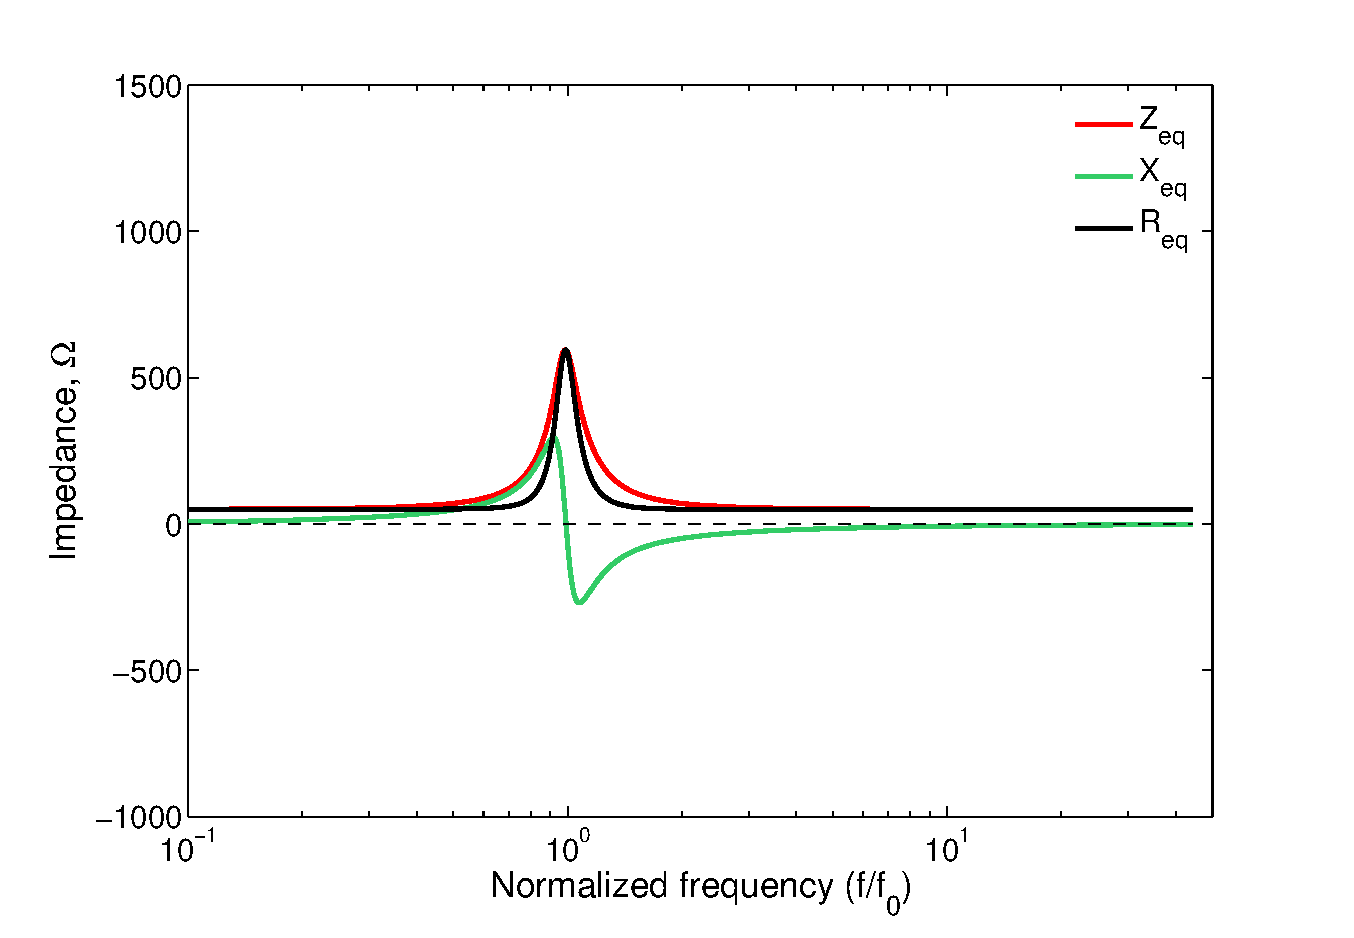
\includegraphics[width=0.7\textwidth]{./images/PS_impedance} 
\caption{Equivalent circuit impedance w.r.t frequency for PS topology}
\end{center}
\end{figure}

\subsubsection{PP topology}

Finally, the PP topology can be obtained through the equations for $Z_R$ and $Z_{eq}$ listed in Appendix \ref{sec:secondaryP} and \ref{sec:primaryP} respectively. This topology is well suited to supply a stable secondary load current due to parallel position of the secondary capacitor \cite{meyer}.
In Figure \ref{F:PoutTopologies} this point is verified when the frequency increases from the resonant one.

\begin{figure}[h!]
\begin{center}
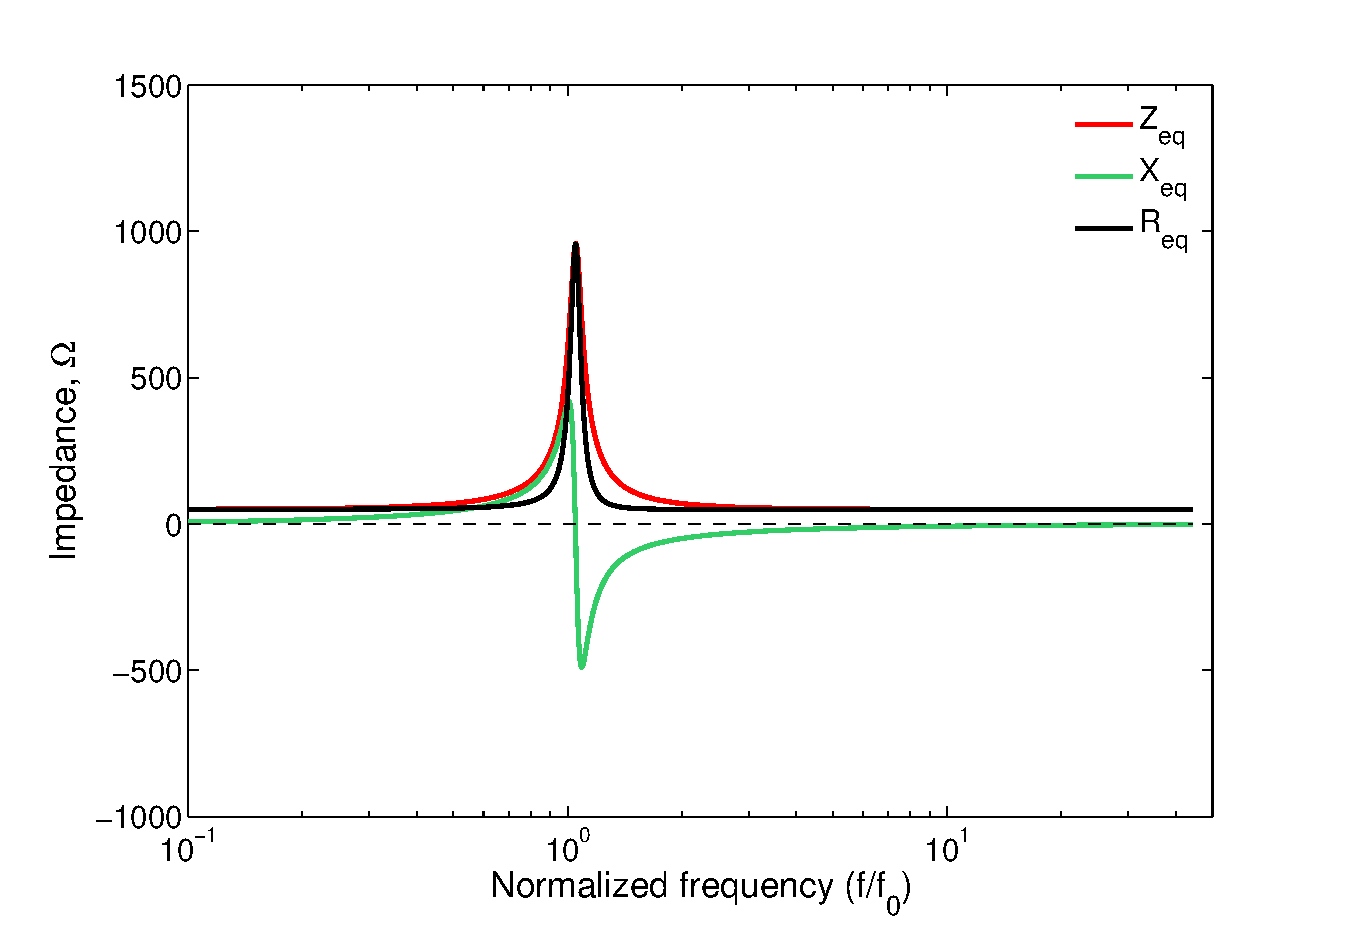
\includegraphics[width=0.7\textwidth]{./images/PP_impedance} 
\caption{Equivalent circuit impedance w.r.t frequency for PP topology}
\end{center}
\end{figure}


The WPT system for this topology will be subjected in the same conditions as in case of the PS topology. Hence, is optimal to drive it with a current source due to its great impedance at the resonance frequency.

\subsubsection{Discussion}\label{subsec:discussion2}

In this section the comparison between each topology is done. The choice of the optimal compensation topology will be made depending on the power levels for a given system load. With the system parameters values, tabulated in Table \ref{T:ArbitraryValues}, the expressions of the efficiency and output power are expressed in Figures \ref{F:effTopologies} and \ref{F:PoutTopologies}. 


\begin{figure}[h!]
\begin{center}
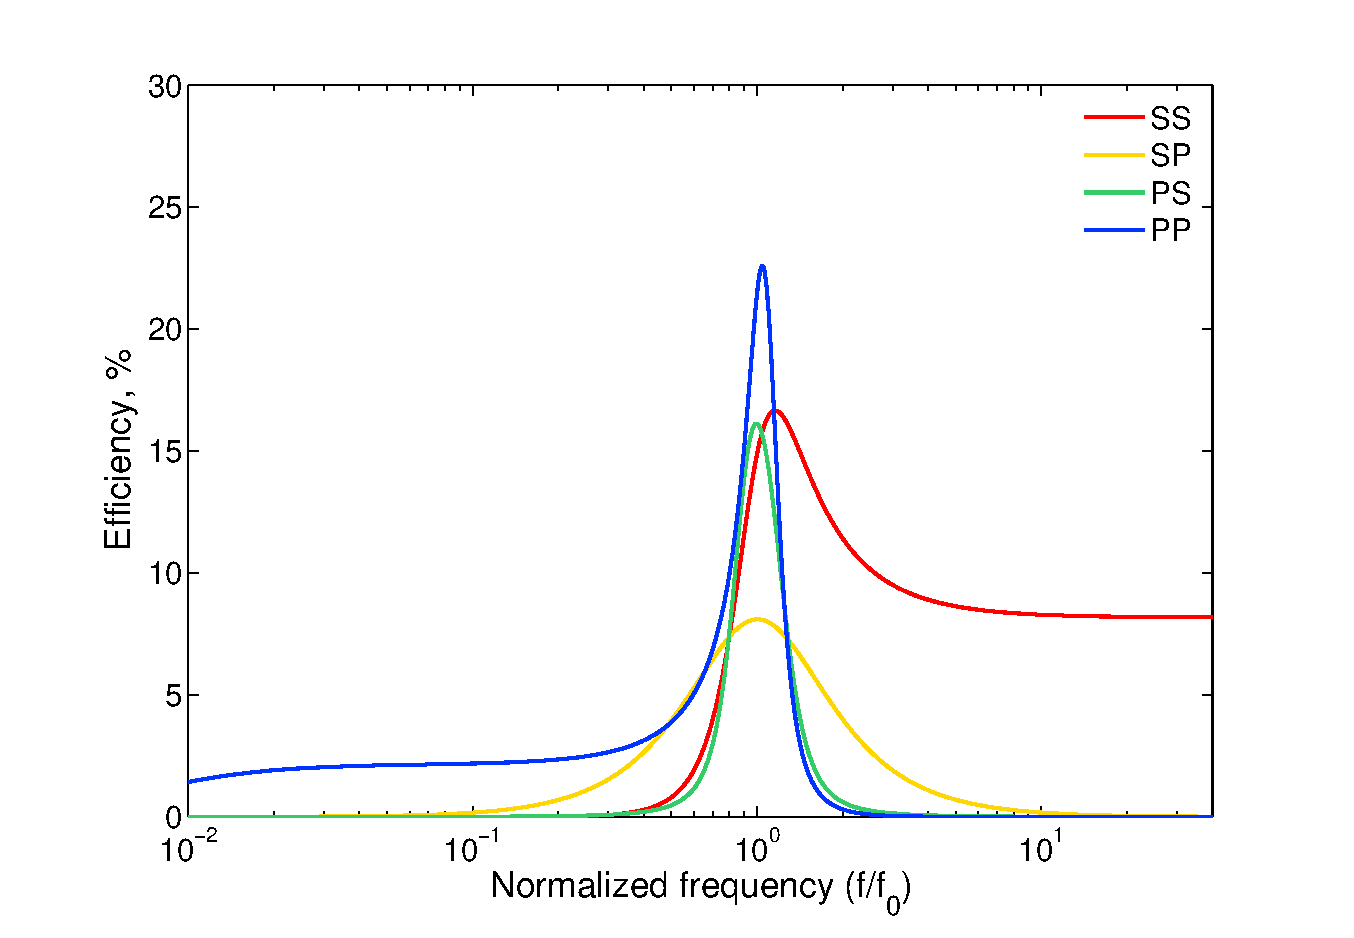
\includegraphics[width=0.7\textwidth]{./images/effModel} 
\caption{Efficiency for all topologies}
\label{F:effTopologies}
\end{center}
\end{figure}

\begin{figure}[h!]
\begin{center}
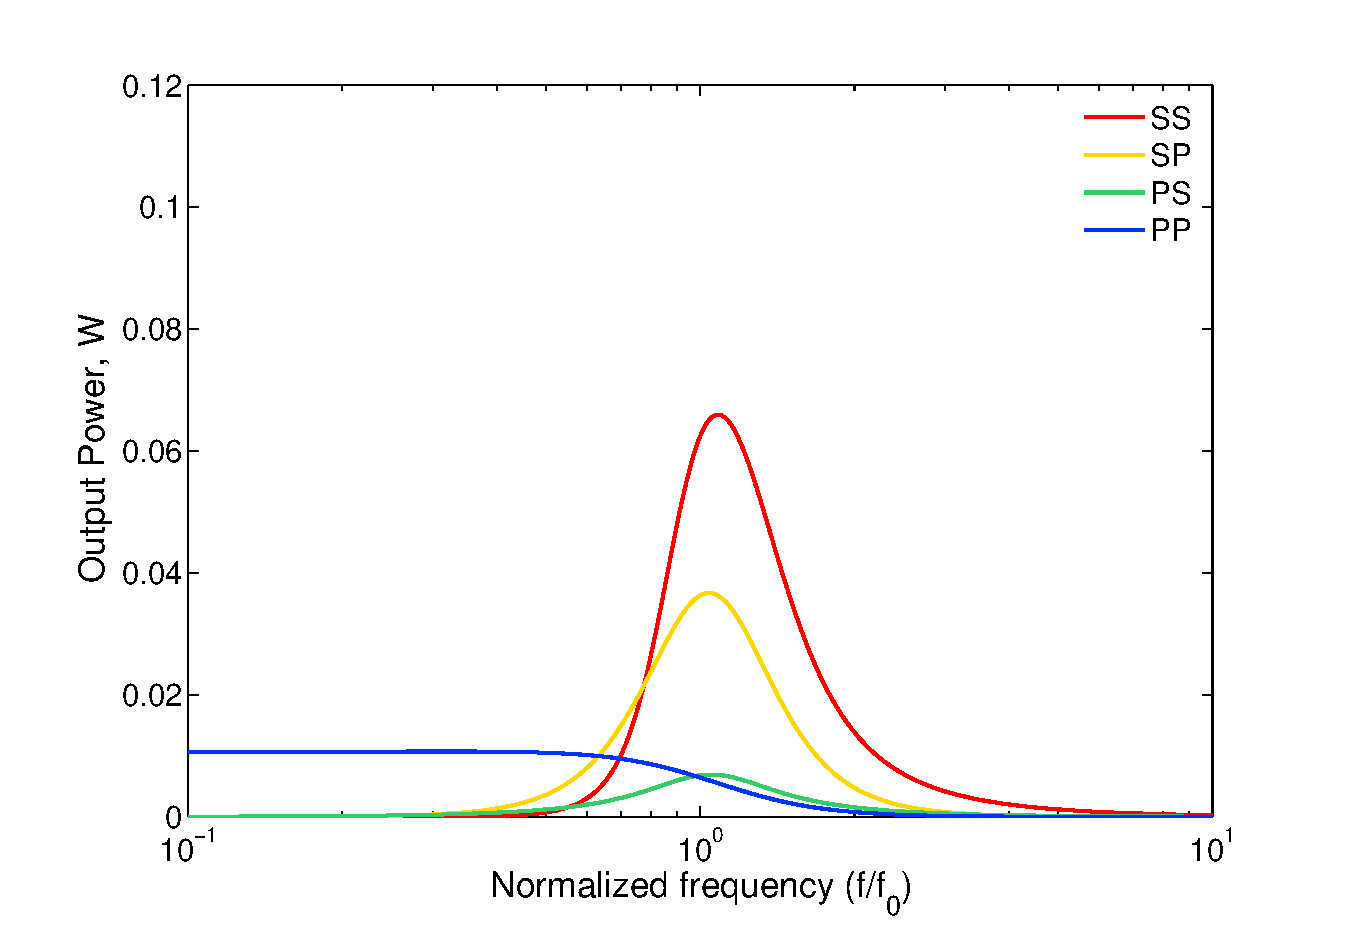
\includegraphics[width=0.7\textwidth]{./images/PoutModel} 
\caption{Output power for all topologies}
\label{F:PoutTopologies}
\end{center}
\end{figure}

The previous figures show that, for the chosen parameters, the optimal topology in terms of output power is the SS topology. The primary series topology has the characteristic that the compensator capacitor does not depend on the load, so it is a good option to select when the loading profile is variable. By comparing the two primary series topologies, when the load becomes higher it is optimal to select a SP topology because the more load resistance, the higher output power levels. This statement can be verified looking at Figure \ref{F:SloadDependance}. 

\begin{figure}[htb]
\begin{center}
\begin{subfigmatrix}{2} 
\subfigure[$R_L = 100\Omega$]
{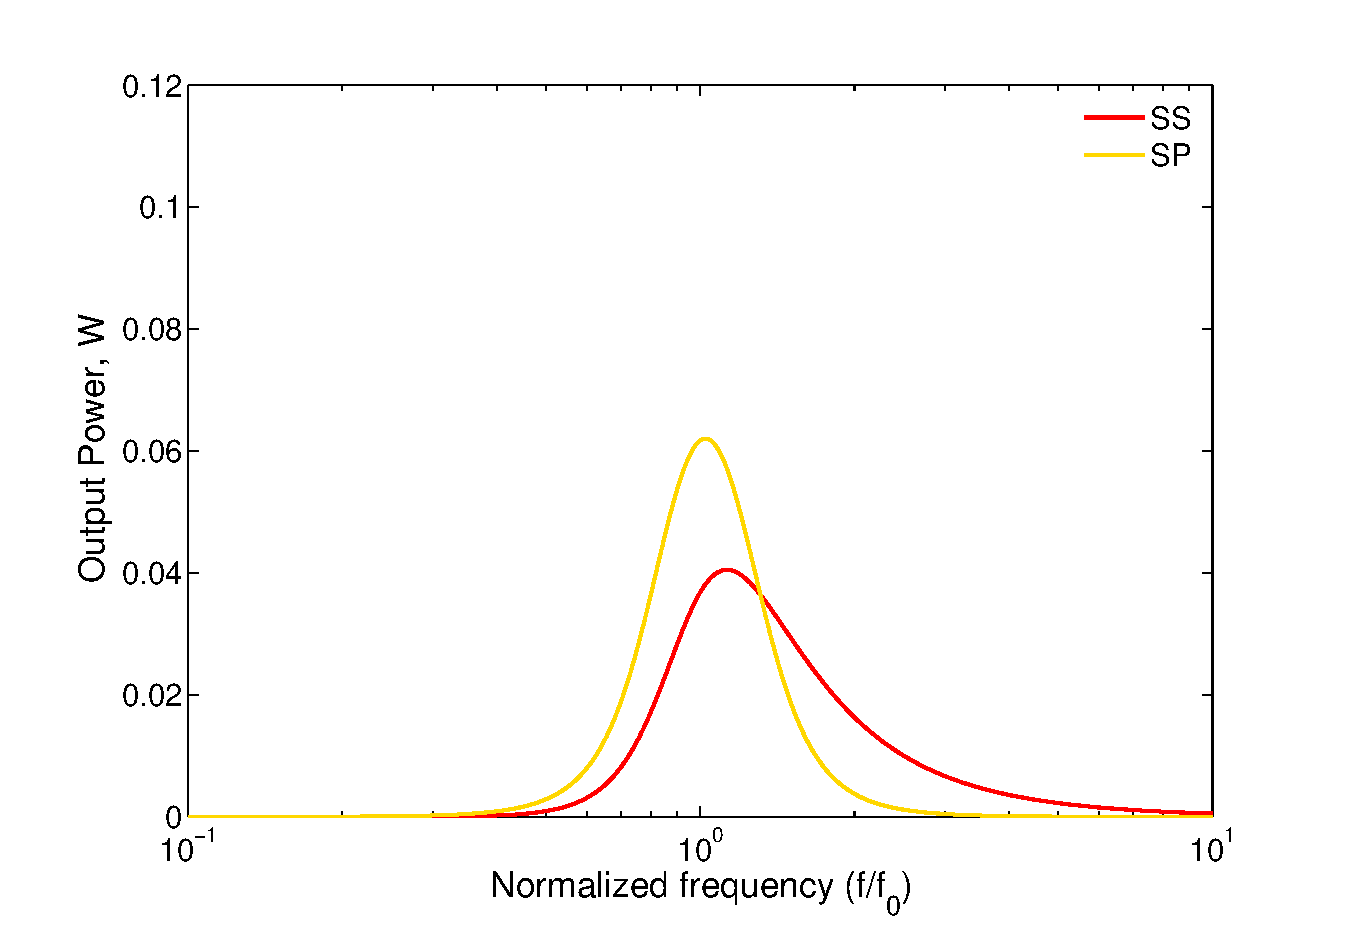
\includegraphics{./images/SS_SP_pout_100}\label{F:S100}} 
\subfigure[$R_L = 1000\Omega$]
{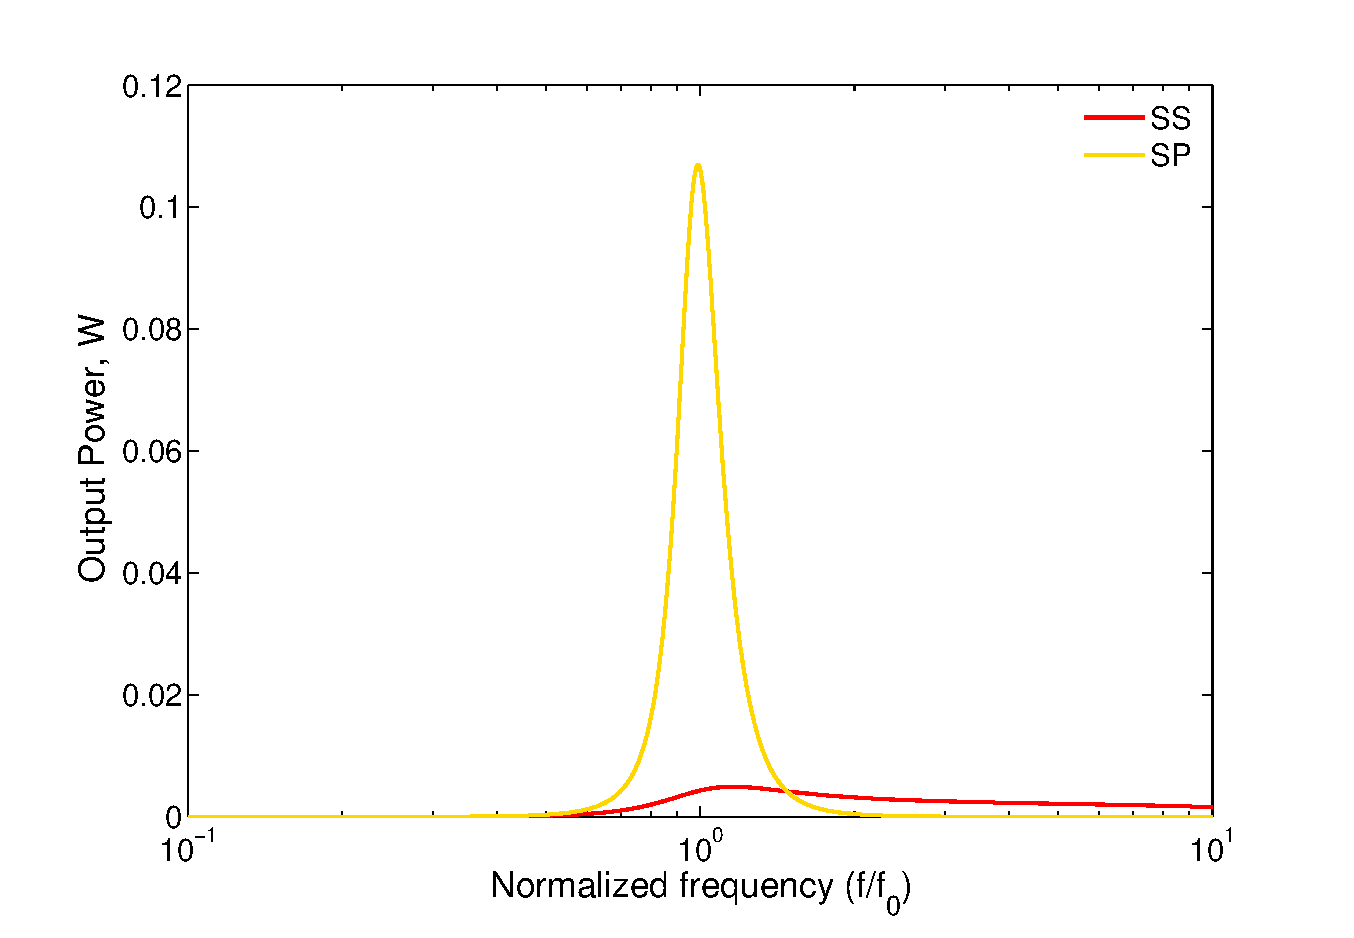
\includegraphics{./images/SS_SP_pout_1000}\label{F:S1000}}
\end{subfigmatrix}
\caption{Output power for SS and SP topologies varying the load resistance}
\label{F:SloadDependance}
\end{center}
\end{figure}

For primary compensated topologies, the compensator capacitor varies with the system load whether is desirable to transfer maximum consumable power at a specific frequency. The output power for these topologies increases when the system load becomes small. In Figure \ref{F:PloadDependence}, the power roughly increases for a PS topology for a small system load but with a lower frequency tolerance. In contrast, a PP topology has a high frequency tolerance in terms of output power. If the system has not a good frequency stability, the best topology to select is the PP topology.

\begin{figure}[htb]
\begin{center}
\begin{subfigmatrix}{2} 
\subfigure[$R_L = 100\Omega$]
{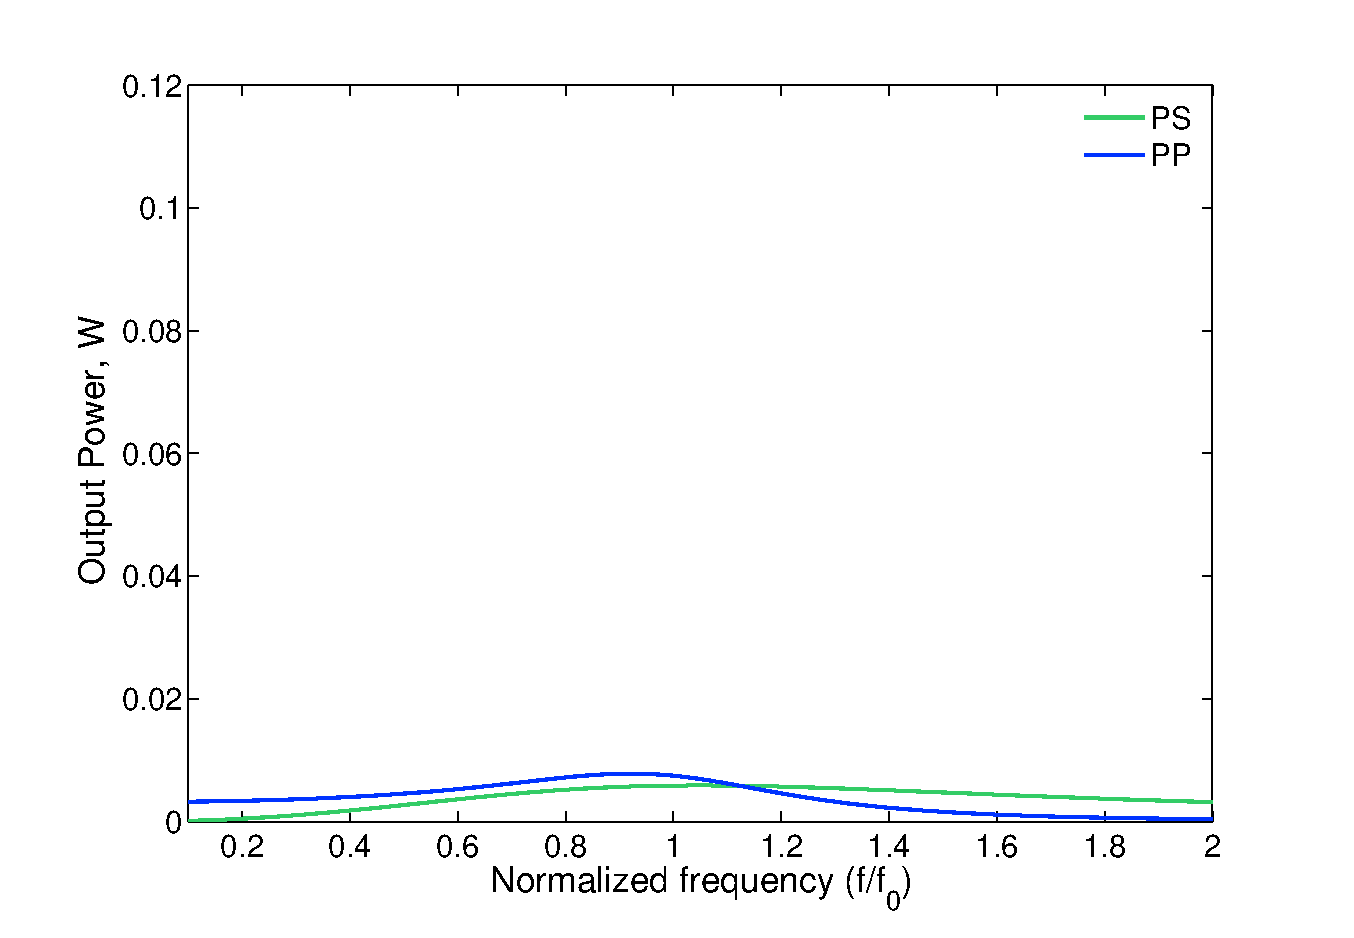
\includegraphics{./images/PS_PP_pout_100}\label{F:P100}} 
\subfigure[$R_L = 1000\Omega$]
{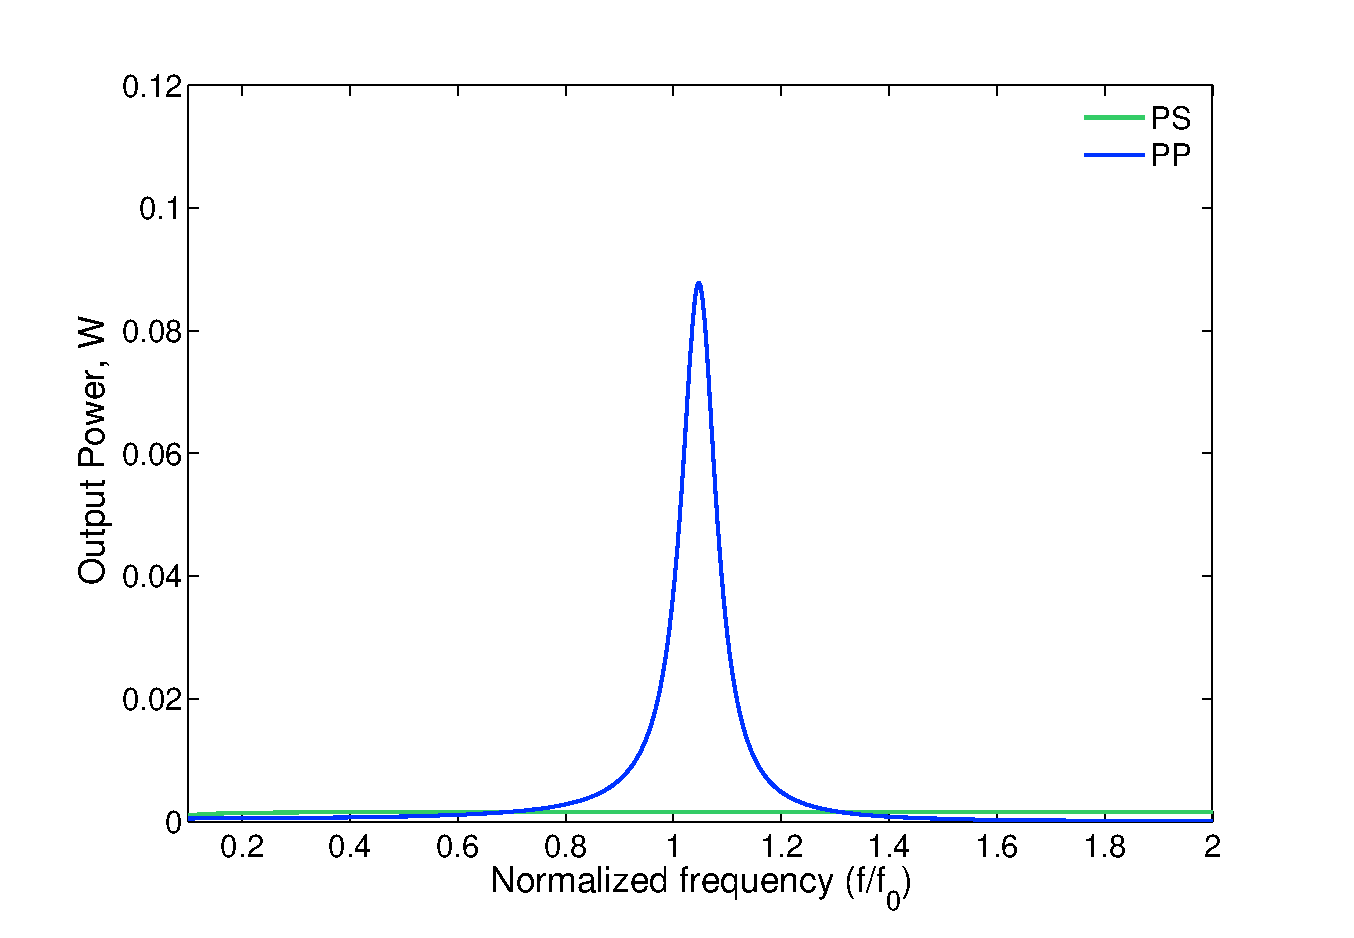
\includegraphics{./images/PS_PP_pout_1000}\label{F:P1000}}
\end{subfigmatrix}
\caption{Output power for SS and SP topologies varying the load resistance}
\label{F:PloadDependence}
\end{center}
\end{figure}

As previous figures show, the worts topology in terms of output frequency is the PS topology. Then, this topology is rejected for using in the studied application. The remaining topologies have good power levels but only one can be selected.

For low load resistances, the better option is the SS topology and is the best manner to transfer energy because both primary and secondary capacitors delete the imaginary parts of impedance allowing to transfer active power. 

When the load resistance increases, secondary parallel capacitors are necessary. To select between SP or PP topologies, we are focused in the effect of the primary capacitors. PP topology generates more amount of reactive power (losses) than SP topology with resonant capacitor, due to the parallel capacitor position on both sides. As a result, the second selected topology is SP topology.

In following sections is discussed the performance of these two topologies and is determined which is the most suitable form to place the compensation capacitors.















	\section{Design Considerations}
Wireless power transfer is a promising way of transfer energy which is said to extend and create new applications restricted in past because of energy issues. By implementing the coupling system on a nano-quadcopter we are trying to enlarge this list of applications. Nevertheless, this attempt of bringing WPT to a new dimension using a nano-quadcopter have involved serious payload constraints.

		\subsection{Power Level}
The power level describes how much power the system is dealing with. We focus on the input and output power of the system, $P_{in}$ and $P_{out}$ respectively, which define induction efficiency. 

\begin{equation}
	\eta = \frac{P_{out}}{P_{in}}
\end{equation}

Although a high power level is not a priority, it is necessary to have at least the boundary power value necessary for running the final application. Whether this power level is higher as the desired it will mean that the distance $z$ (which is referred to the axial distance) could be increased. 

While power level is smaller than expected, it would be necessary to increase at least one of the following parameters in order to rise the transferred power:
\begin{itemize}[noitemsep] % To be more compact --> \begin{itemize}[noitemsep,nolistsep]
	\item Mutual inductance
	\item Voltage induced in the secondary coil
	\item Current through the primary coil 
\end{itemize}

The three parameters are quite related among them. The first one, mutual inductance is strongly dependent on the distance ($M\propto{1/z^3}$). Thus, the first and easiest solution is reduce the axial distance between coils. The second possibility is to increase the induced voltage in the secondary coil, which is proportionally to the operating frequency. Eventually, the magnetizing current through the primary coil can rised by decreasing the operating frequency. This may sound weird since the power transferred can be increased by either decreasing or increasing frequency. A trade-off should be sought to maintain the output power without compromising the transfer distance.

%%
Another important point to consider, once distance and frequency are established, is impedance matching. As we said in Section \ref{subsec:Model} the maximum transfer power occurs when there is an impedance matching between $Z_1$ and $Z_R$. Taking into account that the only variable parameter inside the $Z_R$ expression is the resistance of the load $R_L$, it will be necessary to define the most suitable load value. Note that the reflected impedance depends on $R_L$ and distance, which is expressed by mutual inductance $M$. This lead to define an average value of $R_L$ for an specific range of distances.
%%


% 		\subsubsection{Safety Issues}
% This is closely related to power level. In comparison to wired power systems, WPT systems suffers from unique safety issues. One of the concerns is the risk caused by the expose to electromagnetic radiation. The exposure to low-frequency electric and magnetic fields results in negligible energy absortion and no measurable temperature rise in the body.




		\subsection{Quality Factor}
The quality factor or Q factor is a dimensionless parameter that describes how under-damped a power antenna is; the higher Q factor, the less damping there is. Thus, both \textit{Tx} and \textit{Rx} coils are intended to have great Q factor values because the higher the Q factor are, the higher the transfer efficiency will be \cite{medical}. Q factor at the same time is the response to the previous power trade-off between a higher frequency and therefore higher induced voltage or lower frequency and a greater magnetizing current, and it defined as:

\begin{equation}
	Q = \frac{\omega{L}}{R}=\frac{\omega_0}{\Delta{\omega}}
	\label{eq:Qfactor}
\end{equation}

$Q$ depends on the applied frequency $2\pi{f}=\omega$, the inductance value $L$ and the resistance of the coil $R$. Occasionally radiation resistance $R_{rad}$ is included in the denominator \cite{5413106}. As stated before in Section \ref{subsec:coilResistance} this resistance can be neglected. Q factor also can be seen as a selectivity factor, that is why it is sometimes defined as the quotient of natural frequency $\omega_0$ by the bandwidth $\Delta{\omega}$. 

Q factor is an image of the quality of a given coil. It defines its capacity to generate a large magnetic field and low losses \cite{meyer}. According to \cite{Consortium}, a quality factor below 10 represents a really poor coil that should be avoided for WPT, and values around 100 are excellent for industrial applications. \textit{Good} coils will permit higher operating frequencies, while coils with small Q factor will tend to transfer at lower frequencies as is shown in the next figure.

\begin{figure}[h]
\begin{center}
	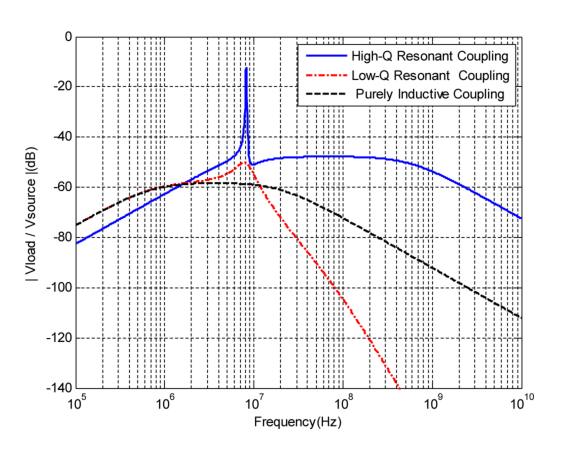
\includegraphics[width=0.7\textwidth]{./images/mit2}
\caption{Voltage transfer function over frequency for different systems}
\label{F:Qfactor}
\end{center}
\end{figure}

From Figure \ref{F:Qfactor} it can be observed three different inductive coupling systems. The high-Q resonant coupling has the highest Q factor, and therefore the narrower bandwidth. Note that in some applications, such as ours, the Q factor is not always the higher, the better. A really high Q factor above 1000, achieved by using open-ended helical coils like in \cite{Karalis200834}, involves a tight bandwidth. Since the resonant frequencies of Tx and Rx coils can not be identically the same, a too narrower band could cause mistuning. In the above figure it can be noticed the huge difference between a pure inductive system and a resonant one. It must be remarked for resonant systems that after their resonant frequency, the overall performance is cut down.


















		\subsection{Coupling Factor}
Together with Q factor, the coupling factor is the most typical parameter to describe air-core transformers. It is expressed as follows:

\begin{equation}
	k = \frac{M}{\sqrt{L_1L_2}}
\end{equation}

This performance parameter measures the fraction of magnetic flux generated by the \textit{Tx} coil is penetrating the \textit{Rx} coil. The more flux reaches the \textit{Rx} coil, the better the two coils are coupled. This level of coupling is expressed by the coupling factor $k$. It varies between 0 and 1. For $k=0$ the two coils are completely decoupled, while the ideal $k=1$ would mean totally coupled coils.

Coupling factor is determined by the size and the position of primary and secondary coils. In Section \ref{subsec:geo} it is discussed the better coils dimension with the purpose to maximize the coupling between them.













		\subsection{Operating Frequency} \label{subsec:operatingFreq}
The operating frequency is another important design consideration in the WPT system. This frequency describes the rate of generation of the electromagnetic waves by the primary coil. For sure, the secondary coil must be designed to work at the operating frequency. As mentioned earlier in Section \ref{subsec:seriesResonance}, to work at resonance it is necessary to drive the primary coil from an external source, in our case it will be an oscillator the responsible of producing the periodic sine wave, \textit{oscillating} at the same operating frequency.

Determine the ideal operating frequency is not possible without knowing many factors as, coil sizes, Q factors, self-resonant frequency, efficiency, etc. Hence, it is intended to determine the suitable frequency band in which the coils could work properly. This frequency range takes into account either the upper and lower frequency boundaries. 

The upper limit is restricted by the maximum switching frequency of the transmitter power driver (red dashed line in Figure \ref{F:frequency}). Another limitation at high frequencies is the one related to coil self-resonance frequency ($f_s$), and so the parasitic capacitance of the coils. Initially any coil is designed to work at $f_s$ to provide the highest possible Q factor. 

Exciting the windings with an excitation frequency of approximately 10$\%$ of $f_s$ will ensure that the parasitic capacitive effects will not influence the inductor impedance values, and that the parasitic capacitances can be removed from the inductor model shown in Figure \ref{F:modelingCoil} \cite{tesis}. Owing to the fact that the experimental results of $f_s$ are not higher than 30 MHz, the maximal operating frequency is set to be at least 5 times lower than the self resonance frequency, as follows,

\begin{equation}\label{eq:maxop}
f\leq\frac{f_s}{5}
% f\simeq\frac{f_s}{5}
\end{equation}

For low frequencies there are no restrictions, but recommendations. The \textit{Wireless Power Consortium} suggests as admissible, Q factor values above 100 for WPT applications. To achieve the desired Q factor, frequencies higher than 500 kHz are typically needed.

\begin{figure}[h]
\begin{center}
	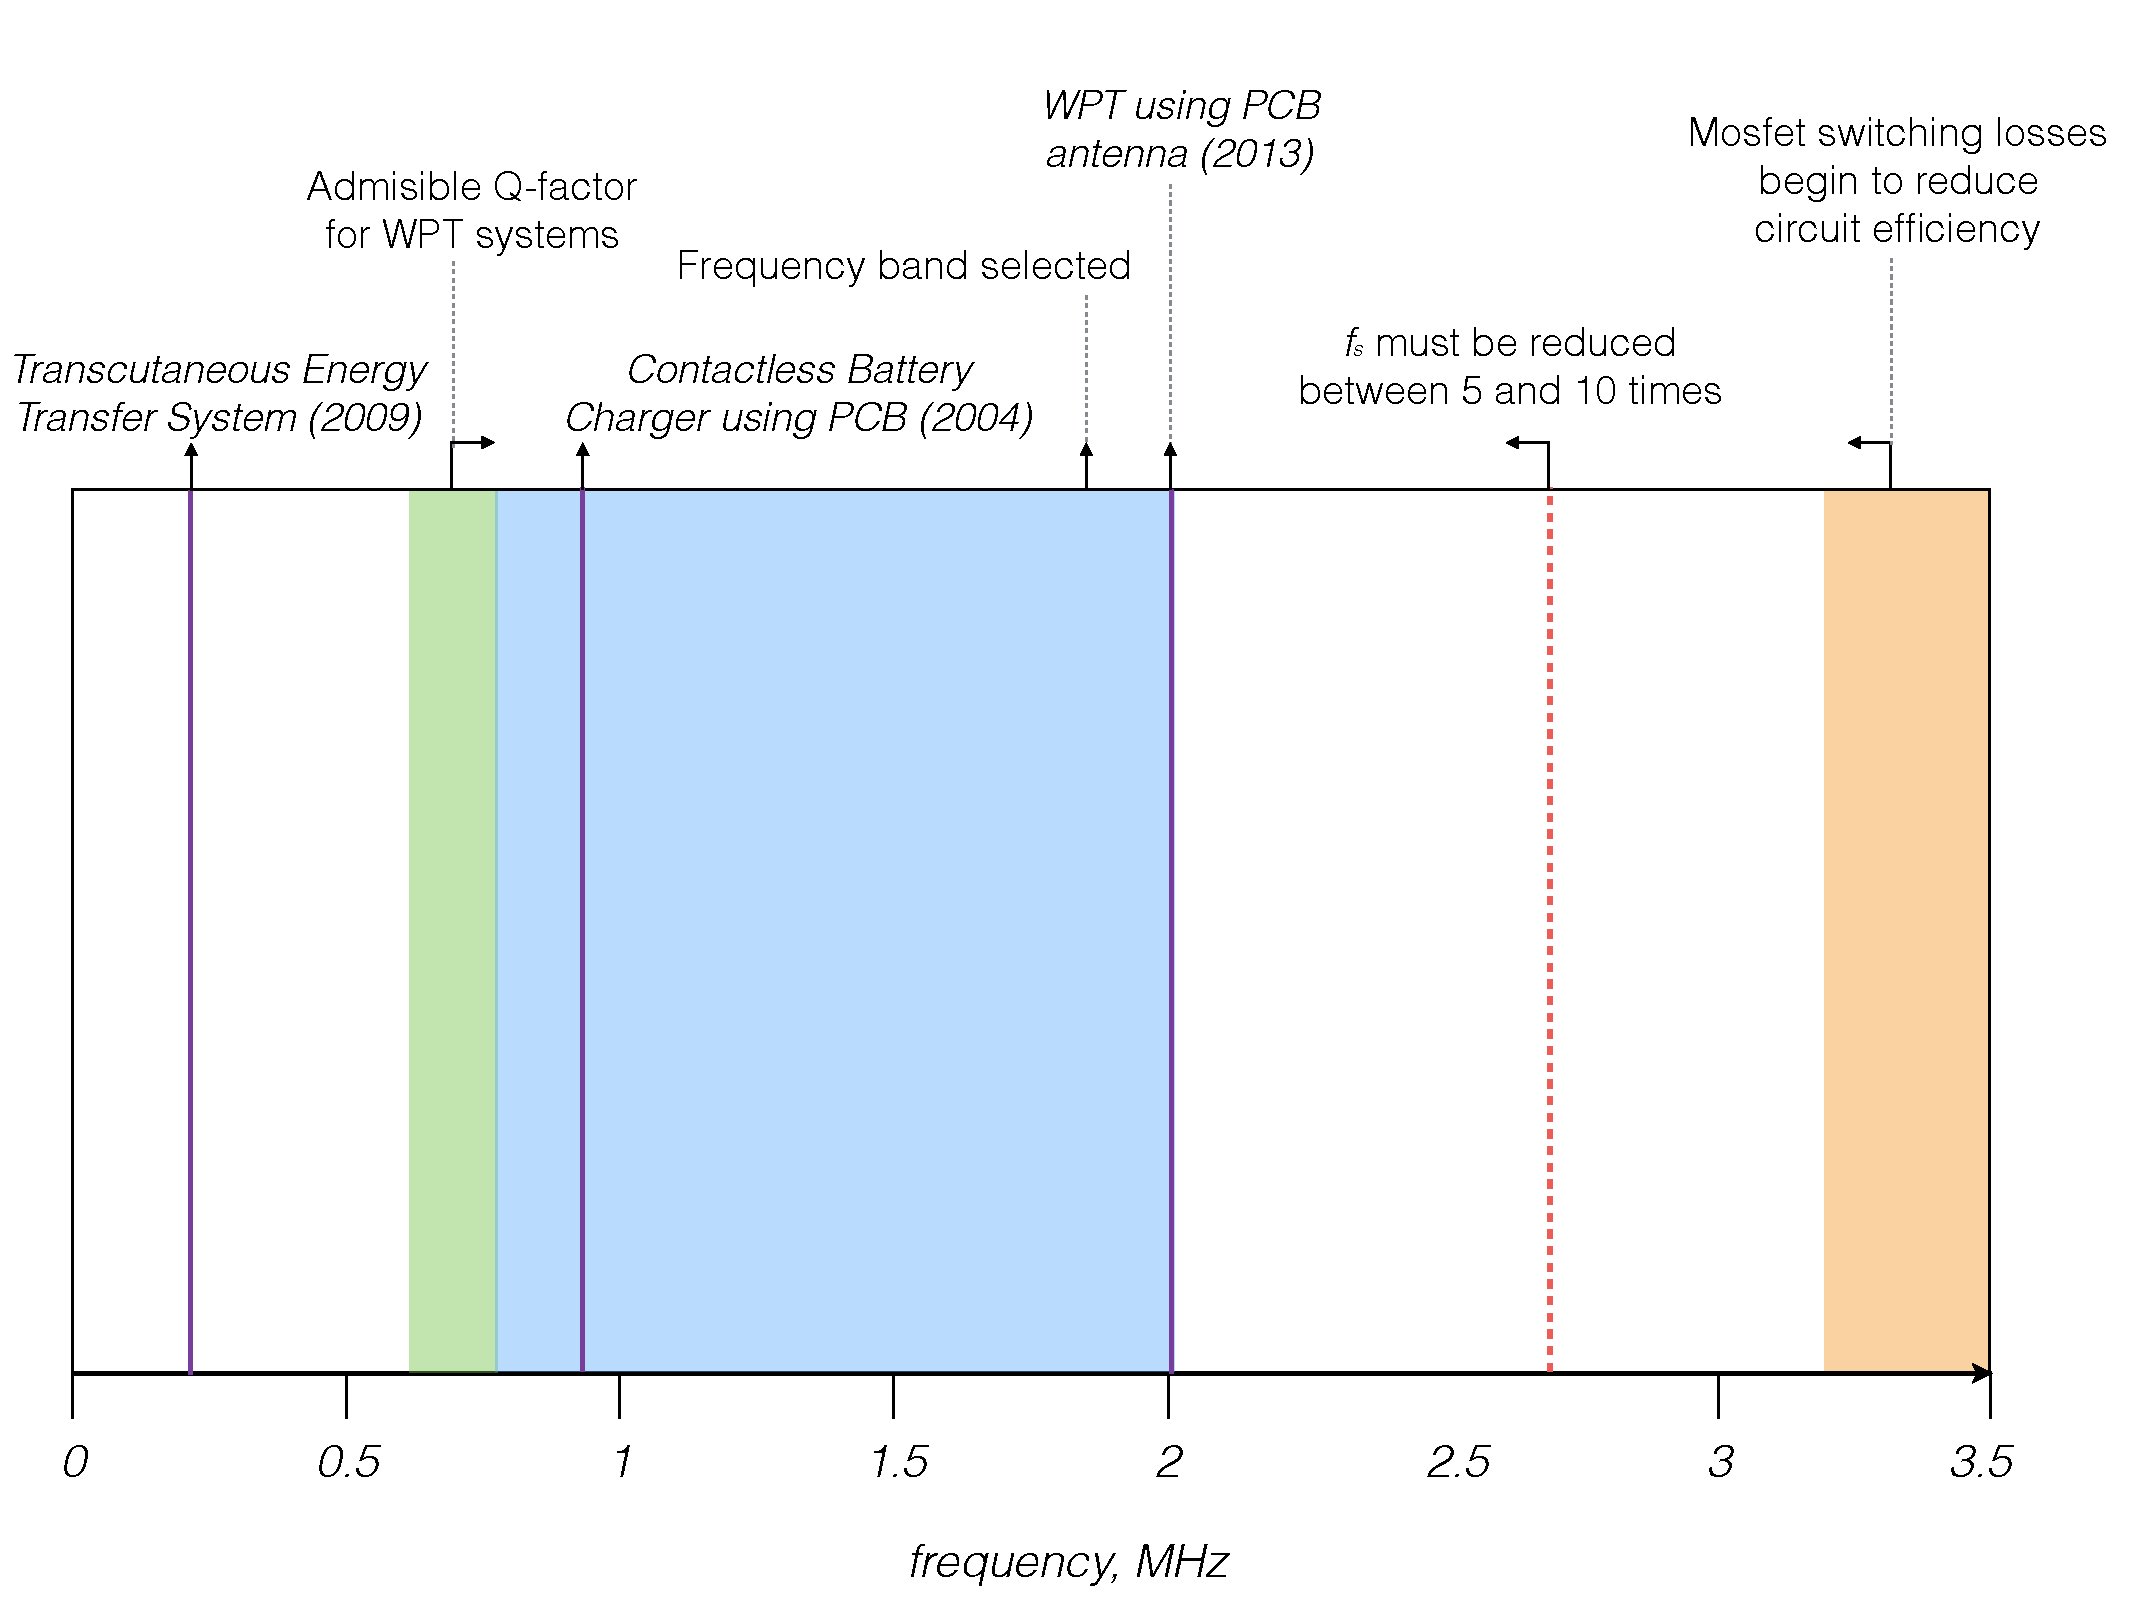
\includegraphics[width=0.95\textwidth]{./images/frequency}
% \vspace{-1.5em}
\caption{Frequency band constraints}

\label{F:frequency}
\end{center}
\end{figure}

Figure \ref{F:frequency} shows the specific frequency band for coils' diameters between 3 and 10 cm which is the desired order of magnitude of the coils. The vertical purple lines indicate different\footnote{Transcutaneous Energy Transfer System \cite{keynote1}, Contactless Battery Charger using PCB \cite{keynote2} and WPT using PCB antenna \cite{keynote3} are useful examples to consider when selecting the operating frequency.} works based on WPT systems similar as ours in terms of transfer distance and coil sizes.

Having set the frequency boundaries and some WPT example applications, for this work the frequency band between 700 kHz and 2 MHz is studied for the next proposed systems.












\subsection{Size and Weight} 
In order to study the behaviour of coils depending on the different coil parameters, such as coil diameter, number of turns, metal conductor or conductor diameter, different models have been designed and tested.

Before knowing power specifications, coil outfitting supports or drone's stability limitations we began to design the power coils. Using a nano-quadcopter as carrying system and resonant induction as mean of power transfer, we set a goal in transferring power up to 20 cm. We chose these range of distances based on previous works \cite{TypicalL}\cite{UAV}\cite{flowchart}\footnote{All the publications selected are similar with regards to operating frequency.}. In front of a design with at least four freedom degrees we decided to fence each variable to reduce the number of possible coil designs.

\begin{table}[ht]
\begin{center}
\begin{tabular}{|c|c|}

\noalign{\global\arrayrulewidth1pt}
\hline
\textbf{Parameter} 	& 	\textbf{Definition}\\
\hline
\hline
$R$ 		& Coil radius		\\ \hline 
$D$  		& Coil diameter		\\ \hline
$A$ 		& Coil area 		\\ \hline 
$d$  		& Wire diameter		\\ \hline 
$l$  		& Wire length		\\ \hline
$S$ 		& Wire section		\\ \hline 
$h$ 		& Coil height		\\ \hline
$z$			& Axial distance	\\ \hline
$N$			& Number of turns 	\\ \hline
$m$			& Coil mass 		\\ \hline  
\end{tabular}
\caption{Geometric parameters of coil models.}
\label{T:coil parameters}
\end{center}
\end{table}

				\subsubsection{Coil Shape}
Winding shape is the most common type of sorting coils. Typical shapes of WPT inductors include circular, square, rectangular and all regular polygons. Whether all these shapes are compared for a given size of the inductor area, it is seen that circular coils obtain a higher magnetic coupling than any other shape. This can be explained by the distorsion of the field distribution around the corners of those shapes \cite{7_Optimized_Magnetic_Design}. Using circular coils we ensure to have the higher possible efficiency. 

				\subsubsection{Metal Conductor}
Each conductor has a different electrical resistivity which is an important parameter to define its DC and AC resistance. This defines the metal used to produce the coils. The following table shows the electrical resistivity of common metal conductors at $20\,^{\circ}{\rm C}$.

\begin{table}[ht]
\begin{center}
\begin{tabular}{|l|c|}
\hline 
Electrical resistivity of Aluminum 	& \rule{0pt}{2ex} $2.44\cdot{10}\textnormal{ x }10^{-8}(\Omega\cdot\textnormal{m})$ \\ \hline
Electrical resistivity of Gold 		& \rule{0pt}{2ex} $1.72\cdot{10}\textnormal{ x }10^{-8}(\Omega\cdot\textnormal{m})$ \\ \hline 
Electrical resistivity of Copper 	& \rule{0pt}{2ex} $1.68\cdot{10}\textnormal{ x }10^{-8}(\Omega\cdot\textnormal{m})$ \\ \hline
Electrical resistivity of Silver	& \rule{0pt}{2ex} $1.59\cdot{10}\textnormal{ x }10^{-8}(\Omega\cdot\textnormal{m})$ \\ \hline
% \rule{0pt}{2ex} --> Superscript does not touch the \hline
\end{tabular}
\caption{Electrical resistivity of several common metal conductors}
\label{T:electricalResistivity}
\end{center}
\end{table}


At first sight silver seems the best conductor due to it has the lowest electrical resistivity and consequently lowest internal resistance at room temperature, but the huge price difference between silver and copper is not worth for only an increase of 5$\%$ in electrical resistivity. Silver is approximately 140 times more expensive than copper \cite{terman1943radio}. As a result, the power coils are made of copper.



				\subsubsection{Conductor Diameter}\label{subsec:diameter} % Cross-sectional area
This paremeter is strongly related with skin effect, discussed in Section \ref{subsec:coilResistance}, and therefore wire resistance. It was analysed whether for the same coil height $h$, fixing the main radius $R$, it was advisable to maximize the number of turns or wire diameter.

Figure \ref{F:Lvsd} shows that for smaller wire diameter, e.g. $d$=0.5 mm and $N$=20 turns, a bigger inductance (Equation \ref{Eq:Harold}) value is achieved in comparison to any other configuration with the same $h$, such as $d$=1 mm and $N$=10 turns. It seems to be better for coil Q factor to reduce wire section, but as always it is a compromise. As Figure \ref{F:skinDepth} shows, decreasing wire diameter we are increasing coil resistance. This effect is most notorious for high frequencies. Hence, it is necessary to ``wait'' for quality factor values.

As stated previously in \ref{subsec:coilResistance} to obtain a good wire performance, the minimum wire diameter will be five times the skin depth $\delta$. Hence, above 1 MHz the minimum diameter will necessary be at least 47 $\mu$m.  

\begin{figure}[htb]
\begin{center}
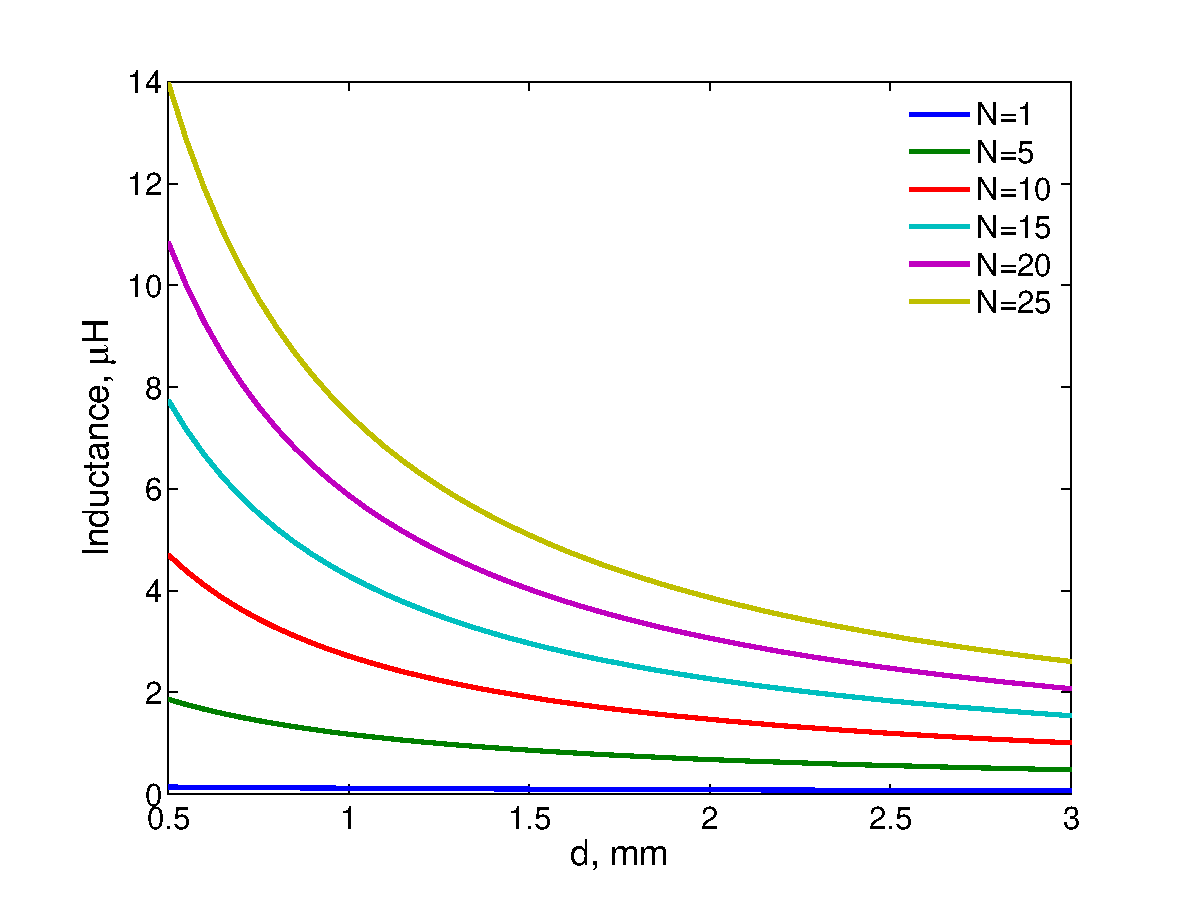
\includegraphics[width=0.6\textwidth]{./images/Lvsd}
\caption{Inductance w.r.t. wire diameter for fixed coil radius of 4 cm and different turns}
\label{F:Lvsd}
\end{center}
\end{figure}

Due to commercial availability we select two different wire diameter, displayed in the following table:

\begin{table}[h]
\begin{center}
\begin{tabular}{|c|c|c|}

\noalign{\global\arrayrulewidth1pt}
\hline
\textbf{Wire diameter} 	& 	\textbf{Insulation} & 	\textbf{Total diameter}\\
\hline
\hline
1 mm		& Polymeric varnish & 	$\sim{}${1 mm}		\\ \hline 
0.59 mm 	& Polymeric layer	& 	1.4 mm 				\\ \hline

\end{tabular}
\caption{Wire diameter}
\label{T:varnish}
\end{center}
\end{table}








				\subsubsection{Number of turns}
First, we determine the maximum number of turns for the quad-copter in 20 turns. This number did not compromise the drone stability in its vertical axis because does not change at all the gravity center. Having a wire reference maximum diameter of 1.4 mm, it means that the largest coil of 20 turns will have 2.8 cm of height, even less height than the quadcopter.

\begin{figure}[htb]
\begin{center}
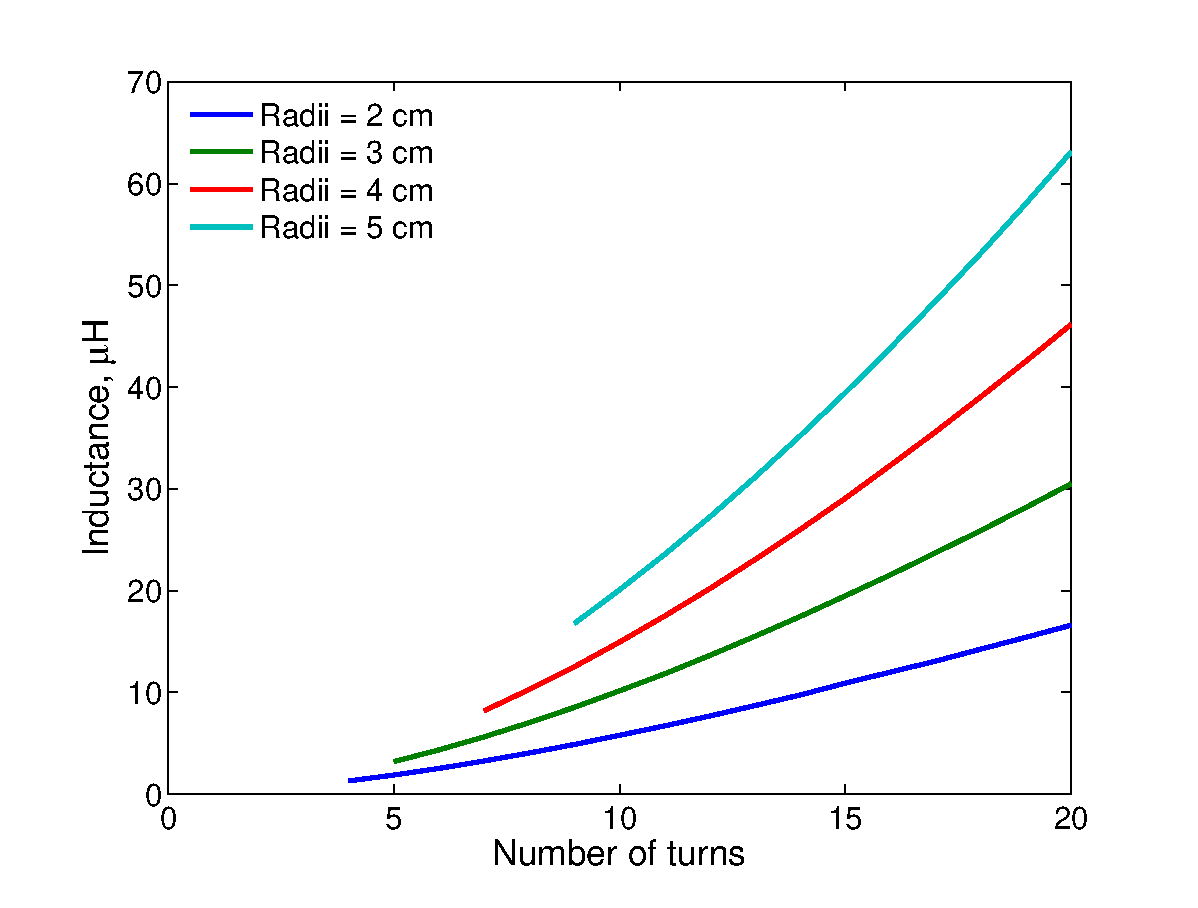
\includegraphics[width=0.6\textwidth]{./images/LvsN}
\caption{Calculated inductance for different number of turns and coil radii values}
\label{F:LvsN}
\end{center}
\end{figure}

Figure \ref{F:LvsN} shows coil inductance depending on the number of turns and on the radius. As the number of turns is increased, coil inductance rises proportionally. In addition, for the same number of turns, higher inductance values are obtained whether the coil radius is increased. It is observed that plotted lines tend to move to the right. This effect is caused by the interpolation method used in this graph, which does not provide higher $D/h$ values from the reference table \cite{WaiKaiChen}. Initially, an increase in coil's radius appears to improve the quality factor of the coil which is a desired purpose. Regrettably we are again in a trade-off situation. By increasing the number of turns we are also increasing the total wire length. This results in a lower quality factor knowing that it is inversely proportional to coil resistance (Equation \ref{eq:Qfactor}). It must be mentioned here that coupling factor does not depend on the number of turns.









				\subsubsection{Coil radius}\label{subsec:geo} %\subsection{Geometrical constraints}
As we said in \ref{sec:discussion}, midrange WPT applications contain distances from coil diameter up to ten times the coil diameter. Thus, if we aspire to transfer power up to 20 cm, at least, a coil with 2 cm of diameter is needed. To design such a smaller coil was refused because it involved imprecise winding, and obviously the smaller the coil area, the smaller magnetic flux is created (\ref{flux}). On the contrary, a great area will imply to have an unbalanced drone which is not designed for carrying oversized objects. The increase in coil area probably will turn into an overall weight-gain.

Furthermore, it has been studied the relation between \textit{Tx} and \textit{Rx} coil area. An axial distance between coils several times the coil radius implies a very small coupling factor $k$ which can be around 0.01 \cite{lowCouplingFactor}. Taking into account that coupling factor lies between 0 and 1, this low value means that only a small amount of the flux generated by \textit{Tx} coil links the \textit{Rx} coil. 

The dashed line set in 0.05 m on the vertical axis means the maximum \textit{Tx} radius allowable owing to the nano-quadcopter dimensions.

\begin{figure}[htb]
\begin{center}
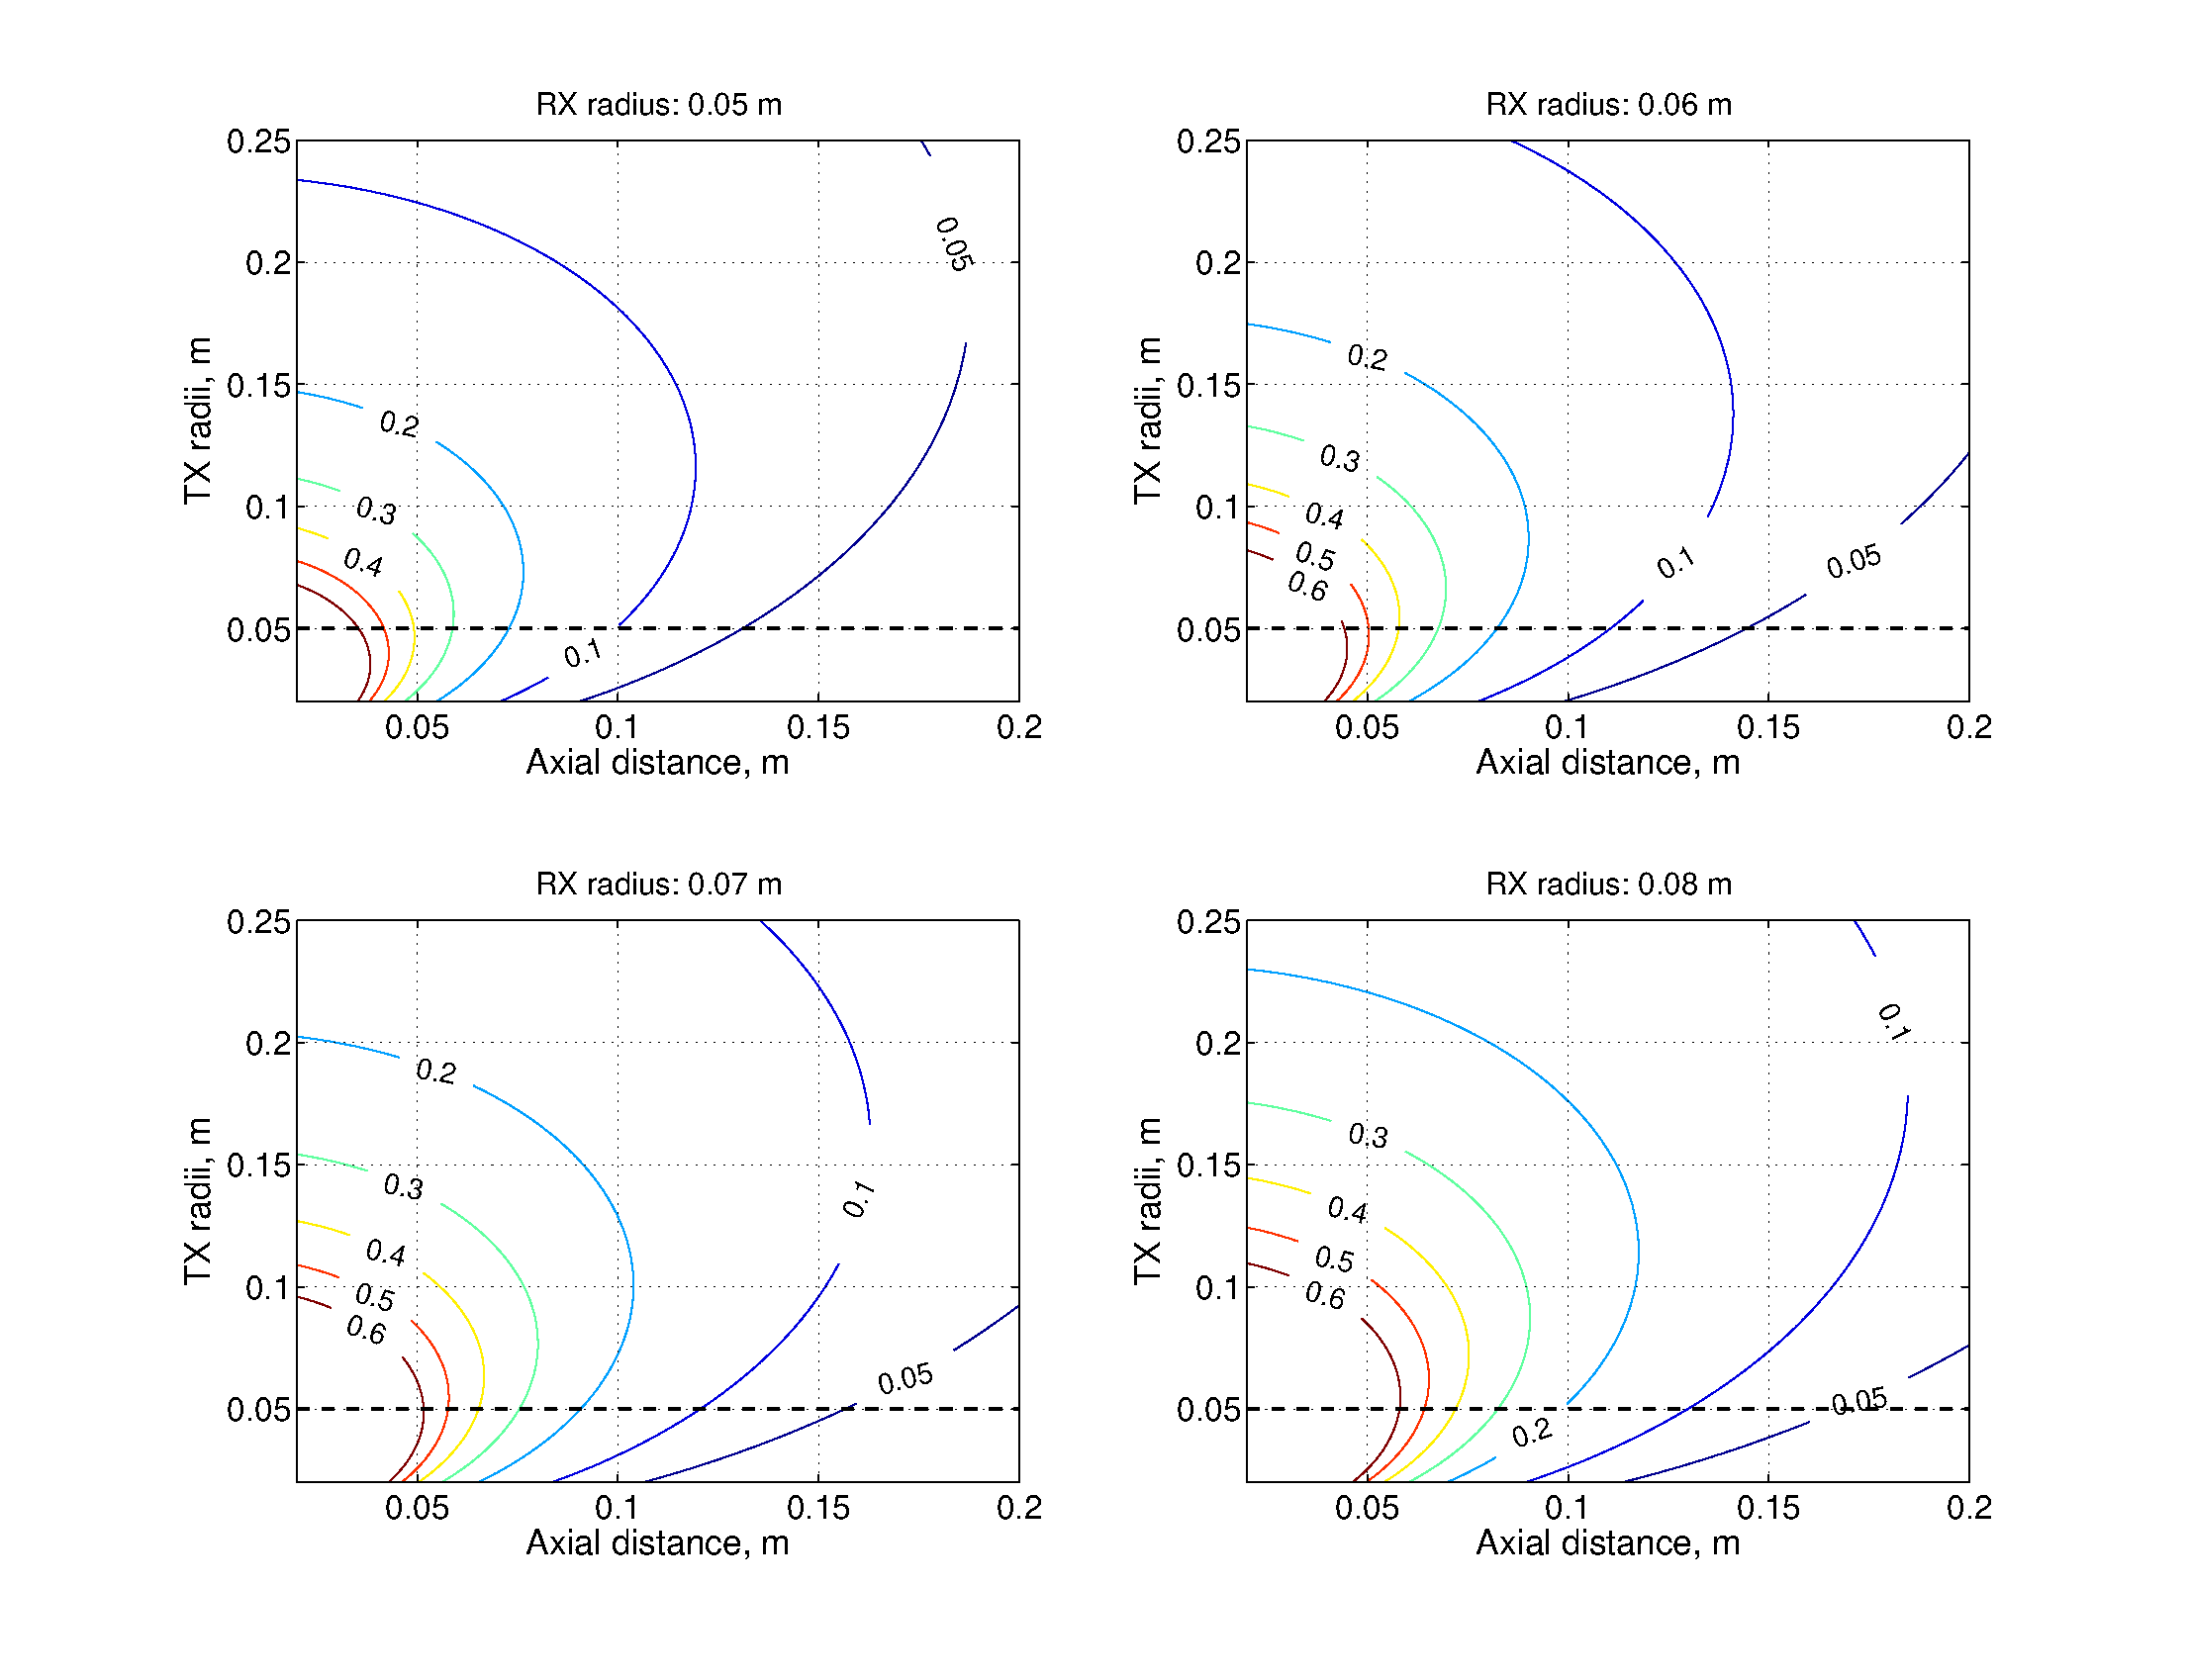
\includegraphics[width=1\textwidth]{./images/contourLines2}
\caption{Contour lines of the magnetic coupling obtained for different distances}
\label{F:contourLines}
\end{center}
\end{figure}

Contrary to common assumption, for larger air gaps the maximum of the magnetic coupling $k$ can not be reached with coils of equal size \cite{7_Optimized_Magnetic_Design}. Figure \ref{F:contourLines} shows the contour lines of the magnetic coupling factor for different air distances and transmitter coil radii for four receiver coil radii. In this case, it has been used the Equation \ref{Eq:typical} to calculate inductances.

It can be shown that bigger \textit{Rx} coils radii improve the coupling factor between the coils, meanwhile increasing \textit{Tx} coil radius does not involve achieving higher $k$ factor. This can be seen with the following example; for a given air gap distance, $z = 0.1$ m, and a fixed \textit{Rx} radius, $R_{RX} = 0.05$ m, by increasing \textit{Rx} radius in 3 cm we see that the coupling factor doubles its value from 0.1 to 0.2. However much \textit{Tx} radius is increased, it will never be possible to duplicate $k$ for the chosen axial distance.  
		
			\subsubsection{Weight} % by default
The \textit{Crazyflie 2.0} 4 DC-motors give it a maximum take-off weight of 42 g \cite{crazyflie}. Part of this payload must be reserved for the transmission circuit and coil's outfitting supports, so we decide to set the coil mass in about 12 g. It must be said that this limitation only affects to the transmitter side.

% Taking into account that this nano quadcopter weighs 27g its maximum payload is set on 15g. 



%%%%%%%%%%%%%%%%%%%%%%%%%%%%
%%%   					 %%%
%%%   Candidate Models   %%%
%%% 					 %%%
%%%%%%%%%%%%%%%%%%%%%%%%%%%%

		\section{Detailed Designs}\label{finTFG}
With intent to create completely different coils we decided to maximize both the coil area and the number of turns while fixing the other variables. The coil shape was round because of its benefits when creating a magnetic field. A copper wire was chosen for its low electrical resistance, as it was said previously. 

% Three coils were designed using the algorithm shown in Figure \ref{F:coilAlgorithm}. The algorithm was initially thought for a 1 mm wire diameter. It maximizes the coil weight in order to take advantage of the quadcopter performance. This results in two completely different coil designs. The first prioritizes the largest possible radius and so few turns. The second model is designed with the minimum radius, which is defined in subsection \ref{subsec:geo}, and the maximum turns permitted. A third model was created in order to test a mixture model. These ``candidates" will allow us to discern clearly the difference between coils' behaviour.

Three coils were designed using the algorithm shown in Figure \ref{F:coilAlgorithm}. The algorithm is thought for a 1 mm copper wire diameter. It maximizes the coil weight in order to take advantage of the quadcopter performance. This results in two completely different coil designs. Note that all coil possibilities have the same or similar lengths. The first model prioritizes the largest possible radius and so few turns. The second is designed with the minimum radius, which is defined in subsection \ref{subsec:geo}, and the maximum turns permitted. A third model was created in order to test a trade-off model. These ``candidates" will allow us to discern clearly the difference between coils' behaviour.

\begin{table}[ht]
\begin{center}
\begin{tabular}{cccccc}

\noalign{\global\arrayrulewidth1pt}
\hline
\noalign{\global\arrayrulewidth0.4pt}
\textbf{Model name} 	& \textbf{Turns} 	& 	\textbf{Radius} & 	\textbf{Wire diameter} & 	$\bm{D/h}$ \textbf{ratio} & 	\textbf{Tx mass}\\
\noalign{\global\arrayrulewidth1pt}
\hline
\noalign{\global\arrayrulewidth0.4pt}
Model A  & 8 	& 	5 cm 	& 	0.597 mm 	& 	11.9 &	13.4 g\\ \hline 
Model B  & 19 	& 	2 cm 	& 	0.597 mm 	& 	1.5  & 	14.1 g\\ \hline 
Model C  & 10 	& 	4 cm 	& 	0.597 mm 	& 	5.71 & 	13.5 g\\ \hline 
Model D1 & 7 	& 	4 cm 	& 	1 mm 		& 	8    & 	17.3 g\\ \hline 
Model D2 & 11 	& 	1.5 cm  & 	1 mm 		& 	2.73 & 	9.8 g\\ \hline 

\end{tabular}
\caption{Geometric parameters of coil models}
\label{T:coil Models}
\end{center}
\end{table}

Both \textit{Tx} and Rx coils were designed with the same dimensions for each of the models A, B and C. This assumption simplifies future computations and also provides us with an added ease for the coil winding procedure. Anyway, we build the last two single-models $D1$ and $D2$ in order to demonstrate the theoretical calculations, which state that an increment in \textit{Rx} radius is preferred upon the same increment in \textit{Tx} radius. 

All the experimental results are carried out for wire of 1.4 mm of diameter, but including its covering (0.59 mm without covering). In this manner we take into account the increase in mass because of the thermal epoxy adhesive inclusion. The wire diameter reduction does not affect since it does still not surpass the boundary stated skin depth, $d>5\delta$. Thus, we ensure not to surpass the maximum payload after adding the adhesive fixation, using a ``lighter'' wire owing to a reduction in the cross-sectional area. In addition, the parasitic capacitance of the coil is reduced due to wire plastic layers, and therefore more space between wires.



% While producing the coils we realized that copper coils of 1 mm of diameter exceeded in mass because of the thermal epoxy adhesive inclusion. Therefore, all the experimental results are carried out for wire of 1 mm of diameter, but now including its covering (0.59 mm without covering). This reduction does not affect since it does still not surpass the boundary stated skin depth, $d>5\delta$. Thus, we ensure not to surpass the maximum payload using a ``lighter'' coil owing to a reduction in the cross-sectional area. In addition we reduce the parasitic capacitance of the coil because of the inclusion of plastic layers, and therefore more space between wires.
% \hfill \break
\begin{figure}[H]

\begin{center}
\begin{tikzpicture}[node distance=2cm]
\vspace{-2em}
	% Define labels
	\node (start) [startstop] {Coil candidate};
	\node (in1) [io, below of=start] {$R_{ini}$\\$N_{ini}$};
	\node (pro1) [process, below of=in1] {Increase $N$};
	\node (pro2) [process, below of=pro1] {Increase $R$};
	\node (dec1) [decision, below of=pro2, yshift=-1.0cm] {$R>$ 5 cm?};
	\node (dec2) [decision, below of=dec1, yshift=-2.0cm] {$m>$ 12 g?};
	\node (end) [startstop, below of=dec2, yshift=-1.0cm] {Store candidate};
	
	% Locate weird labels
	% \node [label={[shift={(-2.2,-4.1)}]$R_{ini}$}] {};
	\node [label={[shift={(-2.2,-6.1)}]$R_{ini}$}] {};
	\node [label={[shift={(-0.4,-11.1)}]No}] {};
	\node [label={[shift={(-0.4,-15.4)}]No}] {};

	% Draw vertical arrows
	\draw [arrow] (start) -- (in1);
	\draw [arrow] (in1) -- (pro1);
	\draw [arrow] (pro1) -- (pro2);
	\draw [arrow] (pro2) -- (dec1);
	\draw [arrow] (dec1) -- (dec2);
	\draw [arrow] (dec2) -- (end);

	% Draw weird arrows
	\draw [arrow] (dec1.west) node[above left]   {Yes} -- + (-15mm,0) |- (pro1.west);
	\draw [arrow] (dec1.west) node[above left]   {} -- + (-15mm,0) |- (pro2.west);
	\draw [arrow] (dec2.west) node[above left]   {} -- + (-14.65mm,0) |- (pro1.west);
	\draw [arrow] (dec2.west) node[above left]   {Yes} -- + (-14.65mm,0) |- (pro2.west);
	\draw [arrow] (end.east) node[above right]   {} -- + (+15.65mm,0) |- (pro2.east);
	% \draw [arrow] (end.east) node[above right]   {} -- + (+15.65mm,0) |- (pro1.east);

\end{tikzpicture}
\end{center}
\caption{Flowchart of the algorithm to design the coil size}
\label{F:coilAlgorithm}
\end{figure}


		\subsection{Discussion}
The decision of which coil model will be outfitted on the quadcopter is based on two criteria: performance and stability. Performance is related with the ability of transfer energy from the source to the load, and so the power transferred and the efficiency. In spite of the fact that the performance has been studied in detail selecting the best compensation topology, in this project the main goal is intended to transfer power, hence the efficiency will not be a decisive parameter.

The second and not less important criteria has to do with weight and shape. Having all the models similar weight it will be determinant to see how does each model behaves, together with the quadcopter. 

It will be necessary to wait until experimental tests to decide which coil is the most suitable. Then, according to the chosen model, it will be set one or other operating frequency.

In Chapter \ref{C:experimental}, all models are tested and compared with theoretical results. It will also be demonstrated that model C is the most appropriate model for transferring power. 

% , we opt for model C for being the most adequate in shape and for working in conjunction with the quadcopter. Model A has a radius too small for landing maneuvers. On the contrary, model B has a radius bigger than the quadcopter complicating the coil support. 




% \begin{table}[ht]
% \centering
% \begin{tabular}{|c|c|c|c|c|c|}

% \noalign{\global\arrayrulewidth1pt}
% \hline
% \textbf{Model name}  &   \textbf{Inductance} 	&   \textbf{Resistance} 	&   \textbf{Q factor} 	&   \textbf{Capacitor}  \\
% \hline
% \hline
% % \tablefootnote{The low inductance and resistance values of model A are due to weight restriction. Model A is a 23\% shorter than other models. By winding one turn involved to exceed mass constraint. Bigger diameters required more adhesive fixation.}

% Model A 	& 7.62$\mu$H 	& 0.489$\Omega$   & 	97 		& 31 nF     \\ \hline 
% Model B  	& 12.72$\mu$H 	& 0.619$\Omega$   & 	129 	& 31 nF 	\\ \hline
% Model C 	& 13.26$\mu$H 	& 0.651$\Omega$   & 	127 	& 31 nF 	\\ \hline

% \end{tabular}
% \caption{Theoretical coil calculations for a test frequency of 1 MHz}
% \label{T:theoretical}
% \end{table}

 



